\documentclass[12pt,a4paper]{report}

% =====================================================
% GÓI HỖ TRỢ TIẾNG VIỆT
% =====================================================
\usepackage[utf8]{inputenc}
\usepackage[T5]{fontenc}
\usepackage[vietnamese]{babel}

% =====================================================
% ĐỊNH DẠNG TRANG
% =====================================================
\usepackage[a4paper,top=2.5cm,bottom=2.5cm,left=3cm,right=2cm]{geometry}
\usepackage{setspace}
\onehalfspacing
\usepackage{indentfirst}
\setlength{\parindent}{1.5em}

% =====================================================
% ĐỒ HỌA, BẢNG BIỂU
% =====================================================
\usepackage[table]{xcolor}
\usepackage{graphicx}
\usepackage{array}
\usepackage{booktabs}
\usepackage{multirow}
\usepackage{caption}
\usepackage{float}
\usepackage{tabularx}
\usepackage{longtable}

% =====================================================
% TOÁN HỌC
% =====================================================
\usepackage{amsmath}

% =====================================================
% MỤC LỤC, LIÊN KẾT
% =====================================================
\usepackage[titles]{tocloft}
\usepackage[
    colorlinks=true,
    linkcolor=black,
    urlcolor=blue,
    citecolor=blue
]{hyperref}

% =====================================================
% ĐỊNH DẠNG CHƯƠNG
% =====================================================
\usepackage{titlesec}

% Định dạng số thứ tự chương (La Mã) và phần (Ả Rập)
\renewcommand{\thechapter}{\Roman{chapter}}
\renewcommand{\thesection}{\arabic{chapter}.\arabic{section}}
\renewcommand{\thesubsection}{\thesection.\arabic{subsection}}

\titleformat{\chapter}[block]
{\normalfont\bfseries\large\centering}
{\MakeUppercase{\chaptertitlename}\ \thechapter.}
{0.5em}
{\MakeUppercase}

\titleformat{\section}[block]
{\normalfont\bfseries\normalsize}
{\thesection.\ }
{0.5em}
{}

\titleformat{\subsection}[block]
{\normalfont\bfseries\normalsize}
{\thesubsection.\ }
{0.5em}
{}

% =====================================================
% MỤC LỤC (CẤU HÌNH TOCLOFT)
% =====================================================
\renewcommand{\cftchapfont}{\bfseries}
\renewcommand{\cftchappagefont}{\bfseries}
\renewcommand{\cftchapleader}{\cftdotfill{\cftdotsep}} % Hiện dấu chấm lửng cho chương

% Định dạng chương trong mục lục: Chương I. TÊN CHƯƠNG
\renewcommand{\cftchappresnum}{Chương\ }
\renewcommand{\cftchapaftersnum}{.}
\setlength{\cftchapnumwidth}{2.5cm}

% Định dạng phần trong mục lục: 1.1. Tên phần
\renewcommand{\cftsecaftersnum}{.}
\setlength{\cftsecnumwidth}{1.2cm}

\renewcommand{\cftsubsecaftersnum}{.}
\setlength{\cftsubsecnumwidth}{1.5cm}

% Lệnh tùy chỉnh để gom hình và bảng chung một trang
\makeatletter
\newcommand{\customlistoffigures}{%
    \section*{\listfigurename}%
    \@starttoc{lof}%
}
\newcommand{\customlistoftables}{%
    \section*{\listtablename}%
    \@starttoc{lot}%
}
\makeatother

% =====================================================
% HEADER / FOOTER
% =====================================================
\usepackage{fancyhdr}

\pagestyle{fancy}
\fancyhf{}
\fancyhead[L]{\small Báo cáo môn Quản lý dự án phần mềm}
\fancyhead[R]{\small \thepage}
\renewcommand{\headrulewidth}{0.4pt}

% =====================================================
% CÁC LỆNH TÙY CHỈNH
% =====================================================
\newcommand{\blankpage}{
    \newpage
    \thispagestyle{empty}
    \null
    \newpage
}

\newcommand{\coverpage}{
    \thispagestyle{empty}
    \pagenumbering{gobble}
}

\setcounter{tocdepth}{2}

% =====================================================
% BẮT ĐẦU TÀI LIỆU
% =====================================================
\begin{document}

% Đánh số hình, bảng, phương trình theo chương
\numberwithin{figure}{chapter}
\numberwithin{table}{chapter}
\numberwithin{equation}{chapter}

% =====================================================
% TRANG BÌA
% =====================================================
\coverpage

\begin{titlepage}
\begin{center}

{\large \textbf{BỘ KHOA HỌC VÀ CÔNG NGHỆ}}\\[0.3cm]
{\large \textbf{HỌC VIỆN CÔNG NGHỆ BƯU CHÍNH VIỄN THÔNG}}\\[0.2cm]

\rule{0.7\textwidth}{0.5pt}\\[0.4cm]


\includegraphics[height=3.5cm,keepaspectratio]{images/ptit-icon.png}\\[0.4cm]

{\Large \textbf{BÁO CÁO}}\\[0.2cm]
{\LARGE \textbf{ĐỒ ÁN MÔN HỌC}}\\[0.2cm]
{\large \textbf{Quản lý dự án phần mềm}}\\[0.6cm]

\begin{minipage}{0.9\textwidth}
\centering
{\Large \textbf{
ĐỀ TÀI:\\[0.3cm]
DevFlow - Hệ thống quản lý dự án phần mềm tích hợp Git, CI/CD và trợ lý AI
}}
\end{minipage}

\vfill

\begin{flushleft}
\hspace{2.2cm}
\begin{minipage}{0.75\textwidth}
\textbf{Môn học:} Quản lý dự án phần mềm\\[0.3cm]
\textbf{Giảng viên hướng dẫn:} Lý Tuấn Anh\\[0.3cm]
\textbf{Thực hiện bởi nhóm sinh viên:}\\[0.2cm]
1. Lâm Nhật Tiên \hfill Mã SV: N23DCCN198\\[0.2cm]
2. Lê Viết Xuân \hfill Mã SV: N23DCCN069
\end{minipage}
\end{flushleft}

\vfill

{\large \textbf{TP. Hồ Chí Minh, tháng 10/2026}}

\end{center}
\end{titlepage}

% =====================================================
% BÌA PHỤ
% =====================================================
\begin{titlepage}
\begin{center}
{\large \textbf{BỘ KHOA HỌC VÀ CÔNG NGHỆ}}\\[0.3cm]
{\large \textbf{HỌC VIỆN CÔNG NGHỆ BƯU CHÍNH VIỄN THÔNG}}\\[1.5cm]
{\Large \textbf{BÁO CÁO ĐỒ ÁN MÔN HỌC}}\\[0.3cm]
{\large Quản lý dự án phần mềm}\\[1.5cm]
{\LARGE \textbf{DevFlow}}\\[0.3cm]
{\large Hệ thống quản lý dự án phần mềm tích hợp Git, CI/CD và trợ lý AI}
\vfill
\begin{flushleft}
\hspace{2cm}
\begin{minipage}{0.78\textwidth}
\textbf{Giảng viên hướng dẫn:} Lý Tuấn Anh\\[0.4cm]
\textbf{Sinh viên thực hiện:}\\[0.2cm]
1. Lâm Nhật Tiên \hfill N23DCCN198\\[0.2cm]
2. Lê Viết Xuân \hfill N23DCCN069
\end{minipage}
\end{flushleft}
\vfill
{\large TP. Hồ Chí Minh, tháng 10/2026}
\end{center}
\end{titlepage}

% Đánh số trang La Mã cho phần đầu báo cáo
\pagenumbering{roman}

% =====================================================
% BẢNG ĐÓNG GÓP VÀ ĐÁNH GIÁ ĐỒNG ĐẲNG
% =====================================================
\chapter*{BẢNG ĐÓNG GÓP THÀNH VIÊN VÀ ĐÁNH GIÁ ĐỒNG ĐẲNG}
\addcontentsline{toc}{chapter}{Bảng đóng góp thành viên và đánh giá đồng đẳng}
\begin{table}[H]
\centering
\begin{tabularx}{\textwidth}{|c|p{2.7cm}|X|c|}
\hline
\textbf{STT} & \textbf{Thành viên} & \textbf{Nội dung đóng góp / đánh giá} & \textbf{Ký tên} \\
\hline
1 & Lâm Nhật Tiên & \begin{minipage}[t]{\linewidth}\begin{itemize}\setlength{\itemsep}{0.15em}\setlength{\topsep}{0.15em}
\item Phụ trách xác thực, tài khoản, workspace và bảo mật người dùng.
\item Phát triển các chức năng AI: phân rã công việc, hỏi đáp dự án và tích hợp MCP.
\item Tham gia xây dựng hệ thống thông báo và triển khai dịch vụ.
\end{itemize}\textbf{Đánh giá: Hoàn thành tốt công việc.}\end{minipage} & \\
\hline
2 & Lê Viết Xuân & \begin{minipage}[t]{\linewidth}\begin{itemize}\setlength{\itemsep}{0.15em}\setlength{\topsep}{0.15em}
\item Phụ trách cơ sở dữ liệu, API và các chức năng quản lý board, cột và task.
\item Xây dựng giao diện Kanban và đồng bộ board theo thời gian thực.
\item Phát triển tích hợp Git/CI, kiểm thử tích hợp và theo dõi hệ thống.
\end{itemize}\textbf{Đánh giá: Hoàn thành tốt công việc.}\end{minipage} & \\
\hline
\end{tabularx}
\end{table}

% =====================================================
% LỜI CAM ĐOAN VÀ LỜI CẢM ƠN
% =====================================================
\chapter*{LỜI CAM ĐOAN}
\addcontentsline{toc}{chapter}{Lời cam đoan}
Nhóm sinh viên cam đoan báo cáo này được thực hiện trên cơ sở quá trình tìm hiểu, lập kế hoạch và phát triển dự án DevFlow. Các nội dung tham khảo từ tài liệu dự án, bảng Trello và nguồn bên ngoài được trích dẫn trong báo cáo. Các số liệu về tiến độ và kiểm thử được ghi kèm nguồn và thời điểm ghi nhận; mục tiêu kế hoạch được phân biệt với kết quả đã có bằng chứng. Nhóm chịu trách nhiệm rà soát nội dung, bổ sung các bằng chứng bàn giao cuối cùng và ký xác nhận trước khi nộp.

\vspace{1cm}
\begin{flushright}
TP. Hồ Chí Minh, ngày \ldots\ tháng \ldots\ năm 2026\\[0.7cm]
\textbf{ĐẠI DIỆN NHÓM SINH VIÊN}\\[1.5cm]
(Ký và ghi rõ họ tên)
\end{flushright}

\chapter*{LỜI CẢM ƠN}
\addcontentsline{toc}{chapter}{Lời cảm ơn}
Nhóm xin chân thành cảm ơn giảng viên hướng dẫn Lý Tuấn Anh đã định hướng và góp ý trong quá trình thực hiện đồ án Quản lý dự án phần mềm. Nhóm cũng cảm ơn các bạn lập trình viên đã chia sẻ nhu cầu và khó khăn trong quy trình quản lý công việc, Git và CI/CD; những thông tin đó giúp nhóm xác định vấn đề và phạm vi sản phẩm DevFlow. Cuối cùng, nhóm cảm ơn các thành viên đã phối hợp phân tích, phát triển và rà soát các hạng mục của dự án.

% =====================================================
% TÓM TẮT TIẾNG VIỆT VÀ ABSTRACT TIẾNG ANH
% =====================================================
\chapter*{TÓM TẮT ĐỒ ÁN}
\addcontentsline{toc}{chapter}{Tóm tắt đồ án}
Đồ án trình bày công tác khởi tạo và quản lý dự án DevFlow, một nền tảng quản lý công việc hướng tới lập trình viên. Dự án giải quyết sự thiếu đồng bộ giữa bảng công việc với hoạt động Git/CI, thời gian phân tích log lỗi và việc phải chuyển đổi liên tục giữa IDE với công cụ quản lý dự án. Nhóm xác định yêu cầu từ hồ sơ Discovery trên Trello, phân loại phạm vi theo MoSCoW, chia công việc thành WBS và ticket, sau đó lập lộ trình phát triển tăng dần gồm năm sprint trong khoảng 10–12 tuần.

Sản phẩm được thiết kế theo kiến trúc modular monolith gồm các miền định danh, board, Git/CI, AI và notification. Tại thời điểm rà soát báo cáo ngày 28/10/2026, bảng Trello ghi nhận 29 thẻ trong cột Done và 18 thẻ trong Backlog; chưa có thẻ ở To Do, In Progress hoặc In Review. Bằng chứng kiểm thử được lưu cho một mốc trước đó, tại commit 4bf5d17 ngày 15/10/2026, ghi nhận 267 kiểm thử backend không lỗi và frontend build thành công. Các hạng mục triển khai cloud và bộ video/slide bảo vệ vẫn còn trong Backlog, nên báo cáo phân biệt rõ kết quả đã ghi nhận với mục tiêu chưa có bằng chứng nghiệm thu.

Đồ án cho thấy việc quản lý phạm vi, phụ thuộc giữa các module, kiểm thử tích hợp và cập nhật tiến độ có vai trò quan trọng với nhóm nhỏ. Kết quả hiện có là cơ sở để tiếp tục hoàn tất các hạng mục Git/CI, AI, triển khai và nghiệm thu theo thứ tự ưu tiên.

\chapter*{ABSTRACT}
\addcontentsline{toc}{chapter}{Abstract}
This report presents the initiation and project management of DevFlow, a developer-focused project coordination platform. The project addresses the gap between task boards and Git/CI activity, the effort required to inspect long CI failure logs, and the context switching between an IDE and project management tools. The team documented user needs in Trello Discovery, prioritized scope with MoSCoW, decomposed work into a WBS and implementation tickets, and planned phased incremental delivery across five sprints over an estimated 10–12 weeks.

DevFlow is designed as a modular monolith with identity, board, Git/CI, AI, and notification domains. At the report review on 28 October 2026, the Trello board recorded 29 cards in Done and 18 in Backlog, with no cards in To Do, In Progress, or In Review. A test evidence record for commit 4bf5d17 on 15 October 2026 reports 267 backend tests without failures and a successful frontend build. Cloud deployment and the final defense package remain in Backlog; therefore, this report distinguishes documented outcomes from targets that have not yet been accepted.

The project demonstrates the importance of scope control, module dependencies, integration testing, and transparent progress tracking in a small development team. The current implementation and management records provide a basis for completing the remaining Git/CI, AI, deployment, and acceptance work.

% =====================================================
% MỤC LỤC VÀ CÁC DANH MỤC
% =====================================================
\tableofcontents
\clearpage

\chapter*{DANH MỤC TỪ VIẾT TẮT VÀ THUẬT NGỮ}
\addcontentsline{toc}{chapter}{Danh mục từ viết tắt và thuật ngữ}
\begin{table}[H]
\centering
\begin{tabularx}{\textwidth}{|l|l|X|}
\hline
\textbf{Từ viết tắt} & \textbf{Tên đầy đủ} & \textbf{Ý nghĩa} \\
\hline
API & Application Programming Interface & Giao diện lập trình ứng dụng \\
AI & Artificial Intelligence & Trí tuệ nhân tạo \\
CI/CD & Continuous Integration / Continuous Delivery & Tích hợp liên tục / phân phối liên tục \\
DoD & Definition of Done & Tiêu chuẩn hoàn thành \\
FR & Functional Requirement & Yêu cầu chức năng \\
IDE & Integrated Development Environment & Môi trường phát triển tích hợp \\
MCP & Model Context Protocol & Giao thức kết nối công cụ AI với ngữ cảnh và công cụ \\
MVP & Minimum Viable Product & Sản phẩm khả dụng tối thiểu \\
NFR & Non-Functional Requirement & Yêu cầu phi chức năng \\
PaaS & Platform as a Service & Nền tảng cung cấp môi trường triển khai ứng dụng \\
PM & Project Management & Quản lý dự án \\
RACI & Responsible, Accountable, Consulted, Informed & Ma trận trách nhiệm \\
SaaS & Software as a Service & Phần mềm cung cấp như một dịch vụ \\
SDLC & Software Development Life Cycle & Vòng đời phát triển phần mềm \\
SOA & Service-Oriented Architecture & Kiến trúc hướng dịch vụ \\
STOMP & Simple Text Oriented Messaging Protocol & Giao thức nhắn tin dùng cho đồng bộ thời gian thực \\
WBS & Work Breakdown Structure & Cấu trúc phân rã công việc \\
\hline
\end{tabularx}
\end{table}

\customlistoftables
\addcontentsline{toc}{chapter}{Danh mục bảng số liệu}
\clearpage
\customlistoffigures
\addcontentsline{toc}{chapter}{Danh mục hình vẽ và biểu đồ}
\clearpage

% Chuyển sang đánh số trang Ả Rập cho nội dung chính
\pagenumbering{arabic}

% =====================================================
% PHẦN NỘI DUNG CHÍNH
% =====================================================
\chapter{TỔNG QUAN DỰ ÁN VÀ KHỞI TẠO}
\section{Bối cảnh và vấn đề cần giải quyết}
Trong quy trình phát triển phần mềm, thông tin công việc thường nằm rải rác giữa bảng quản lý tác vụ, kho mã nguồn, hệ thống tích hợp liên tục và môi trường lập trình. Khi các công cụ này không được kết nối, thành viên phải cập nhật trạng thái thủ công; bảng công việc có thể không phản ánh kịp hoạt động commit, mở pull request hoặc hợp nhất mã. Khi pipeline kiểm thử thất bại, nhật ký dài cũng khiến việc xác định nguyên nhân mất thời gian. Việc liên tục chuyển giữa IDE và trình duyệt làm gián đoạn quá trình phát triển [1], [3].

Từ những vấn đề đó, nhóm đề xuất DevFlow, một nền tảng điều phối dự án hướng tới lập trình viên. Hệ thống kết hợp bảng Kanban với hoạt động Git và CI/CD, đồng thời cung cấp trợ lý AI để hỗ trợ phân rã công việc, tra cứu thông tin dự án và tóm tắt lỗi. Mục tiêu là giảm thao tác cập nhật lặp lại và giúp thành viên nắm được tình trạng công việc tại cùng một nơi [1], [2].

\section{Mục tiêu, phạm vi và sản phẩm bàn giao}
Mục tiêu dự án là xây dựng một sản phẩm web có thể triển khai trên môi trường cloud, đáp ứng các luồng quản lý công việc cốt lõi và có khả năng tích hợp với quy trình phát triển phần mềm. Hiến chương xác định nhóm gồm hai thành viên, thời gian dự kiến từ 10 đến 12 tuần, tổ chức thành năm sprint. Các con số này là cơ sở lập kế hoạch của dự án, không phải kết quả nghiệm thu [1].

Các mục tiêu chất lượng được đặt ra gồm: giữ ranh giới module và kiểm tra bằng tác vụ xác minh kiến trúc; duy trì thời gian phản hồi P95 cho API CRUD cốt lõi dưới 200 ms; đồng bộ trạng thái bảng qua WebSocket trong dưới một giây; và đạt độ chính xác tóm tắt nguyên nhân lỗi CI/CD từ 90\% trở lên trên bộ kiểm thử. Nhóm cũng đặt mục tiêu áp dụng kiểm tra đầu vào phía máy chủ, xử lý lỗi có cấu trúc, giám sát và cơ chế bảo vệ tài khoản [1], [3]. Đây là các ngưỡng mục tiêu cần được đo và đối chiếu khi nghiệm thu.

Sản phẩm bàn giao dự kiến gồm ứng dụng DevFlow, mã nguồn và cấu hình triển khai, cơ sở dữ liệu cùng các migration, kiểm thử, tài liệu kỹ thuật, hướng dẫn cài đặt và tài liệu trình bày/demo. Phạm vi tính năng được phân loại chi tiết theo MoSCoW ở Chương III.

\section{Các bên liên quan và đối tượng sử dụng}
Các bên liên quan chính gồm nhóm phát triển, giảng viên hướng dẫn và người dùng mục tiêu. Nhóm phát triển chịu trách nhiệm lập kế hoạch, thực hiện, kiểm tra và bàn giao; giảng viên/hội đồng theo dõi và đánh giá kết quả môn học; người dùng mục tiêu cung cấp góc nhìn về nhu cầu và khả năng sử dụng. Hiến chương xác định Tiên Lâm là Project Leader/Project Manager, phụ trách quản trị phạm vi và điều phối chung; Lê Viết Xuân là Technical Co-Lead, tập trung vào board, Git/CI, hạ tầng local và quan sát hệ thống [1]. Phân công kỹ thuật chi tiết được trình bày trong ma trận RACI ở Chương II.

Đặc tả sản phẩm xác định ba nhóm người dùng đại diện: lập trình viên làm việc độc lập cần một công cụ gọn nhẹ; kỹ sư trong nhóm nhỏ cần theo dõi task gắn với commit, pull request và kết quả CI; và tech lead/PM cần nhìn thấy tiến độ thực tế mà không phải phụ thuộc hoàn toàn vào cập nhật thủ công [2], [3].

\section{Tổng quan giải pháp DevFlow}
DevFlow cung cấp bảng Kanban để quản lý board, cột và task; task có thể gắn người phụ trách, hạn hoàn thành, mức ưu tiên và mô tả. Hệ thống dự kiến tiếp nhận sự kiện Git để liên kết nhánh/commit/pull request với task và cập nhật trạng thái theo vòng đời phát triển. Khi CI thất bại, log được chuyển tới năng lực AI để tạo bản tóm tắt. Người dùng có thể hỏi thông tin dự án qua giao diện chat; MCP adapter mở rộng một số năng lực đó tới công cụ AI trong IDE [3], [5].

Theo kiến trúc đã chọn, backend là modular monolith gồm các miền auth, board, gitci, AI và notification. Các module có quyền sở hữu dữ liệu riêng và giao tiếp qua sự kiện miền hoặc hợp đồng API công khai; giao diện web là ứng dụng React, dữ liệu được lưu trong PostgreSQL. Cách tổ chức này giữ sản phẩm trong một dịch vụ triển khai phù hợp với quy mô nhóm, đồng thời đặt ranh giới rõ ràng giữa các miền nghiệp vụ [5].

\section{Điều lệ dự án và tiêu chí thành công}
Hiến chương dự án là căn cứ thống nhất về lý do thực hiện, mục tiêu, phạm vi cấp cao, vai trò, giới hạn và tiêu chí thành công. Theo PMI, project charter chính thức ghi nhận sự tồn tại của dự án và tạo căn cứ quản trị để tổ chức nguồn lực cho công việc [6]. Với DevFlow, Trello ghi nhận hiến chương, phân công trách nhiệm, phạm vi MoSCoW, các mốc dự kiến và Definition of Done; đây là cơ sở để theo dõi các thay đổi trong suốt dự án [1].

Tiêu chí thành công không chỉ là giao diện chạy được. Sản phẩm cần đáp ứng phạm vi đã chốt, qua kiểm thử phù hợp, giữ ranh giới module, xử lý lỗi an toàn và có thể triển khai theo cấu hình mục tiêu. Các ngưỡng về hiệu năng, độ trễ đồng bộ và độ chính xác AI nêu ở mục 1.2 phải có bằng chứng đo kiểm trước khi được xác nhận là đạt [1], [3].

\chapter{MÔ HÌNH VÀ PHƯƠNG PHÁP QUẢN LÝ DỰ ÁN}
\section{Mô hình phát triển được lựa chọn}
Nhóm lựa chọn cách tổ chức phát triển tăng dần theo giai đoạn, chia kế hoạch thành năm sprint và ưu tiên bàn giao từng phần có thể tích hợp. Đây là cách tiếp cận phù hợp với sản phẩm phần mềm có nhiều miền chức năng, nhóm nhỏ và thời hạn học kỳ cố định. Scrum Guide mô tả cách tiếp cận lặp và tăng dần như một phương tiện kiểm soát rủi ro và cải thiện khả năng dự đoán [7]. DevFlow sử dụng sprint làm đơn vị lập kế hoạch; báo cáo gọi phương pháp của dự án là phát triển tăng dần theo giai đoạn, không khẳng định nhóm áp dụng toàn bộ khung Scrum.

Việc chia giai đoạn giúp nhóm sớm tích hợp nền tảng và luồng người dùng cốt lõi trước khi mở rộng sang tự động hóa, AI và phát hành. Sau mỗi giai đoạn, phần mềm, kiểm thử và phạm vi còn lại có thể được xem xét để điều chỉnh thứ tự ưu tiên trong giới hạn đã thống nhất [4].

\section{Quy trình làm việc và các giai đoạn dự án}
Chu trình quản lý một hạng mục gồm: xác định nhu cầu; ghi nhận yêu cầu và tiêu chí chấp nhận; phân rã thành ticket; gán người phụ trách và ưu tiên; phát triển theo nhánh Git; kiểm thử và review; cập nhật trạng thái Trello; sau đó tích hợp vào nhánh chung. Definition of Done trong hiến chương yêu cầu có kiểm thử tự động, kiểm tra dữ liệu phía máy chủ, phản hồi lỗi theo chuẩn dự án và xác minh ranh giới module [1].

Lộ trình cấp cao được Trello xác định như sau [1]:
\begin{enumerate}
    \item \textbf{Sprint 1 — Nền tảng và định danh (2 tuần):} cơ sở dữ liệu ban đầu, xác thực JWT, workspace và giao diện quản lý người dùng.
    \item \textbf{Sprint 2 — Bảng Kanban (2,5 tuần):} dữ liệu board/task, API, kéo thả và đồng bộ WebSocket.
    \item \textbf{Sprint 3 — Git và CI (2 tuần):} tiếp nhận webhook có xác thực, liên kết commit/nhánh với task và tự động cập nhật trạng thái.
    \item \textbf{Sprint 4 — AI và MCP (2 tuần):} tích hợp Spring AI, phân rã task, tóm tắt lỗi, chat và adapter MCP.
    \item \textbf{Sprint 5 — Hoàn thiện và phát hành (1,5 tuần):} gia cố chất lượng, thông báo, giám sát và triển khai cloud.
\end{enumerate}
Thời lượng các sprint trong lộ trình cộng lại khoảng 10 tuần; khung 10–12 tuần trong hiến chương dành phần dự phòng cho tích hợp, sửa lỗi và nghiệm thu [1], [4].

\section{Vai trò, trách nhiệm và cơ chế phối hợp}
Hiến chương phân công theo quyền sở hữu tính năng xuyên suốt, từ backend tới frontend. Ma trận RACI dưới đây tóm tắt trách nhiệm cấp cao; A là chịu trách nhiệm cuối cùng, R là trực tiếp thực hiện, C là được tham vấn và I là được thông tin [1].

\begin{table}[H]
\centering
\caption{Ma trận trách nhiệm RACI cấp cao của dự án}
\begin{tabularx}{\textwidth}{|X|c|c|c|}
\hline
\textbf{Gói công việc} & \textbf{Tiên Lâm} & \textbf{Lê Viết Xuân} & \textbf{GV/Hội đồng} \\
\hline
Quản trị dự án, phạm vi, DoD và hiến chương & A/R & C & I \\
Kiến trúc hướng dịch vụ và Event Bus & A & R & C \\
Module auth và bảo mật JWT & A/R & I & I \\
Module board và đồng bộ WebSocket & C & A/R & I \\
Module gitci và webhook & C & A/R & I \\
Module AI và MCP & A/R & C & I \\
Module notification & A/R & I & I \\
Docker local và Grafana & C & A/R & I \\
Phát hành cloud và nghiệm thu sản phẩm & A/R & R & A (nghiệm thu) \\
\hline
\end{tabularx}
\end{table}

Nhóm sử dụng Trello làm nơi quản lý backlog và trạng thái công việc, Git/GitHub để quản lý mã nguồn và review thay đổi, cùng các công cụ trong repo để kiểm thử và chạy hệ thống. Hiến chương quy định họp rà soát tiến độ hằng tuần; các quyết định ảnh hưởng phạm vi cần được ghi lại để cả hai thành viên cùng nắm [1].

\section{Công cụ quản lý và kiểm soát phiên bản}
Trello lưu hiến chương, kết quả discovery, danh sách ticket, checklist và trạng thái công việc. Các cột của bảng phát triển phân biệt backlog, việc sẵn sàng thực hiện, đang làm, chờ review và hoàn tất. Ticket là đơn vị theo dõi có thể truy về tính năng và đầu ra tương ứng. Nhóm dùng quy ước nhánh `feature/T-XXX-...`, mã ticket trong tên nhánh/commit và Conventional Commits; hiến chương yêu cầu pull request được review trước khi hợp nhất [1].

Git là nguồn quản lý phiên bản và căn cứ để review thay đổi. Docker Compose hỗ trợ khởi chạy môi trường local gồm các dịch vụ của hệ thống; CI chạy kiểm tra tự động cho thay đổi. Prometheus và Grafana được chọn cho quan sát số liệu vận hành theo kế hoạch kiến trúc [4], [5]. Việc dùng các công cụ này không thay thế tiêu chí nghiệm thu: mỗi đầu ra vẫn cần được đối chiếu với ticket, kiểm thử và Definition of Done.

\section{Cơ sở lựa chọn mô hình}
Quy mô hai thành viên và thời hạn một học kỳ khiến việc vận hành nhiều dịch vụ độc lập có thể làm tăng chi phí triển khai, cấu hình và xử lý lỗi phân tán. Vì vậy, kiến trúc modular monolith giảm số thành phần cần vận hành nhưng vẫn giữ ranh giới nghiệp vụ trong code. Lộ trình theo giai đoạn cho phép kiểm soát tích hợp và tập trung nguồn lực vào MVP trước; phân loại MoSCoW giúp nhóm xác định tính năng thiết yếu, tính năng quan trọng, phần có thể làm nếu còn năng lực và nội dung được loại khỏi đợt bàn giao [1], [5], [8].

MoSCoW là kỹ thuật ưu tiên hóa yêu cầu theo bốn nhóm Must Have, Should Have, Could Have và Won't Have this time; hướng dẫn của Agile Business Consortium nhấn mạnh việc phân biệt yêu cầu bắt buộc với yêu cầu có thể trì hoãn khi giới hạn thời gian [8]. Cách áp dụng cụ thể vào DevFlow được trình bày ở Chương III.

\chapter{QUẢN LÝ PHẠM VI DỰ ÁN}
\section{Thu thập và phân tích yêu cầu}
Phạm vi được hình thành từ vấn đề người dùng, phân tích thị trường, hành trình phát triển phần mềm và khả năng thực hiện trong khung 10–12 tuần của nhóm hai người. Hồ sơ Discovery trên Trello xác định các hoạt động thu thập gồm phỏng vấn lập trình viên, lập bản đồ hành trình SDLC, phân tích log CI/CD, xây dựng persona, pain point và kịch bản Jobs-to-be-Done [2]. Đây là cơ sở định hướng yêu cầu; các kết quả khảo sát chi tiết cần được lưu kèm hồ sơ nếu báo cáo cần trình bày số liệu định lượng.

Yêu cầu được chia thành yêu cầu chức năng (hành vi và năng lực sản phẩm) và yêu cầu phi chức năng (chất lượng, bảo mật, hiệu năng, vận hành). Quy trình truy vết của nhóm đi từ nhu cầu người dùng tới giải pháp, module, ticket và kiểm thử; các thẻ Discovery ghi nhận ma trận truy vết từ pain point qua tính năng tới kiến trúc và ticket triển khai [2], [3].

\section{Phạm vi sản phẩm và phạm vi dự án}
\subsection{Phạm vi sản phẩm}
Trong phạm vi sản phẩm là một nền tảng quản lý dự án dành cho lập trình viên với các nhóm năng lực sau:
\begin{itemize}
    \item Quản lý tài khoản, workspace và thành viên; bảo vệ đăng nhập và dữ liệu người dùng.
    \item Quản lý board, cột và task theo Kanban; theo dõi người phụ trách, mức ưu tiên và thông tin task; đồng bộ thay đổi cho nhiều người dùng.
    \item Kết nối hoạt động Git/CI với công việc: nhận webhook, xác định task liên quan, cập nhật trạng thái và hiển thị thông tin build.
    \item Hỗ trợ AI cho phân rã yêu cầu, hỏi đáp thông tin dự án và tóm tắt lỗi CI; cung cấp các điểm truy cập chat/MCP theo phạm vi ưu tiên.
    \item Hỗ trợ thông báo, quan sát vận hành, kiểm thử và triển khai theo các hạng mục được ưu tiên trong Trello.
\end{itemize}

\subsection{Phạm vi dự án}
Phạm vi dự án bao gồm hoạt động quản lý để phân tích, thiết kế, phát triển, kiểm thử, tích hợp và chuẩn bị bàn giao sản phẩm. Các đầu ra quản lý gồm hiến chương, yêu cầu, phân loại MoSCoW, phân rã ticket/WBS, phân công, kế hoạch giai đoạn, tiêu chí DoD, tài liệu kiểm thử, hướng dẫn cài đặt và demo. PMI mô tả WBS là sự phân rã có thứ bậc của toàn bộ phạm vi công việc thành các phần có thể quản lý để tạo ra đầu ra dự án [9]. Do đó, WBS của DevFlow được tổ chức theo nhóm đầu ra như sau:

\begin{enumerate}
    \item Quản trị dự án: charter, discovery, yêu cầu, phạm vi, kế hoạch, rủi ro và tài liệu nghiệm thu.
    \item Nền tảng và định danh: cơ sở dữ liệu ban đầu, tài khoản, xác thực, workspace.
    \item Quản lý công việc: board, cột, task, giao diện Kanban, đồng bộ thời gian thực.
    \item Tích hợp Git/CI: schema, webhook, parser, sự kiện miền, chuyển trạng thái và hiển thị trạng thái.
    \item Năng lực AI và cộng tác: cấu hình AI, phân rã task, hỏi đáp, tóm tắt lỗi, chat/MCP và notification.
    \item Chất lượng và phát hành: kiểm thử, bảo mật, giám sát, Docker, triển khai cloud và tài liệu hướng dẫn.
\end{enumerate}
Các ticket Trello phân rã những nhóm đầu ra này thành các hạng mục kỹ thuật có người phụ trách và checklist; danh sách chi tiết được quản lý trên bảng phát triển [1].

\subsection{Phân loại ưu tiên MoSCoW}
Trello xác định ưu tiên cấp cao như sau [1], [2]:
\begin{itemize}
    \item \textbf{Must Have:} xác thực JWT; board Kanban và đồng bộ thời gian thực; webhook Git có HMAC; liên kết Git với task và tự động chuyển trạng thái; tiếp nhận lỗi CI; tóm tắt CI bằng AI; phân rã task và chat gateway.
    \item \textbf{Should Have:} MCP server cho công cụ AI trong IDE; thông báo trong ứng dụng; dashboard Grafana; audit logging.
    \item \textbf{Could Have:} gom nhóm lỗi CI lặp lại; cảnh báo rủi ro trễ hạn; khởi tạo dự án từ template.
    \item \textbf{Won't Have trong phạm vi hiện tại:} luồng phê duyệt hành chính nhiều cấp; form builder tùy biến; CRM/email marketing; phân quyền doanh nghiệp nhiều tầng; mở rộng tích hợp tràn lan ngoài phạm vi đã chọn.
\end{itemize}
MoSCoW dùng để quản lý thứ tự ưu tiên, không tự động chứng minh một tính năng đã hoàn thành. Trạng thái bàn giao của từng hạng mục cần căn cứ vào ticket, kiểm thử và nghiệm thu [8].

\section{Cấu trúc phân rã công việc (WBS)}
WBS cấp cao dưới đây diễn đạt phạm vi theo đầu ra, từ đó các ticket kỹ thuật được theo dõi trên Trello. Cách phân rã hướng đầu ra phù hợp với mục tiêu WBS là mô tả toàn bộ công việc cần thiết để tạo sản phẩm bàn giao [9].

\begin{table}[H]
\centering
\caption{WBS cấp cao của dự án DevFlow}
\begin{tabularx}{\textwidth}{|c|X|X|}
\hline
\textbf{Mã WBS} & \textbf{Gói công việc} & \textbf{Đầu ra chính} \\
\hline
1.0 & Quản trị và phân tích dự án & Charter, yêu cầu, phạm vi, backlog, kế hoạch và rủi ro \\
2.0 & Nền tảng và định danh & Schema nền tảng, Auth, JWT, workspace \\
3.0 & Bảng quản lý công việc & Board, cột, task, Kanban và đồng bộ thời gian thực \\
4.0 & Tích hợp Git và CI & Webhook, liên kết task, sự kiện, cập nhật trạng thái và trạng thái CI \\
5.0 & AI và cộng tác & Phân rã task, hỏi đáp, tóm tắt lỗi, chat/MCP và notification \\
6.0 & Chất lượng và phát hành & Kiểm thử, bảo mật, giám sát, triển khai và hướng dẫn \\
\hline
\end{tabularx}
\end{table}

\section{Sản phẩm bàn giao và tiêu chí nghiệm thu}
Sản phẩm bàn giao gồm ứng dụng web và backend có thể chạy theo môi trường được cấu hình; schema/migration cơ sở dữ liệu; tích hợp các tính năng nằm trong phạm vi ưu tiên; mã nguồn và lịch sử thay đổi; kiểm thử; tài liệu kiến trúc, cài đặt và sử dụng; cùng bản demo phục vụ nghiệm thu. Trello cũng liệt kê tài liệu trình bày và Definition of Done trong các đầu việc bàn giao [1].

Các tiêu chí nghiệm thu cấp dự án được tổng hợp như sau:
\begin{itemize}
    \item Chức năng bàn giao truy vết được về yêu cầu và ticket đã thống nhất.
    \item Kiểm thử phù hợp được thực thi; lỗi nghiêm trọng được xử lý hoặc ghi nhận rõ.
    \item Kiểm tra ranh giới module không phát hiện phụ thuộc triển khai chéo bị cấm.
    \item API xác thực đầu vào phía máy chủ và trả lỗi theo quy ước; không để lộ chi tiết nội bộ.
    \item Đo và lưu bằng chứng cho mục tiêu hiệu năng API, đồng bộ WebSocket và chất lượng tóm tắt AI đã nêu trong Hiến chương.
    \item Có hướng dẫn chạy/cài đặt và bản demo để giảng viên/hội đồng kiểm tra.
\end{itemize}
Các ngưỡng định lượng là tiêu chí mục tiêu; chỉ kết luận đạt khi có kết quả đo hoặc kiểm thử tương ứng [1], [3].

\section{Quy trình kiểm soát thay đổi phạm vi}
Khi phát sinh yêu cầu mới hoặc thay đổi, nhóm ghi nhận nội dung và lý do trên Trello, xác định yêu cầu liên quan, sau đó phân tích ảnh hưởng tới đầu ra, thời gian, nguồn lực, phụ thuộc kỹ thuật, chất lượng và rủi ro. Nhóm phân loại lại theo MoSCoW; nếu thêm hạng mục mới trong điều kiện thời hạn cố định, cần nêu rõ hạng mục nào được lùi hoặc loại khỏi đợt bàn giao. Sau khi thống nhất, nhóm cập nhật ticket, tiêu chí chấp nhận, WBS và kế hoạch sprint để bảo đảm các tài liệu cùng phản ánh một phạm vi [1], [2], [8], [9].

Các yêu cầu thuộc Won't Have không được đưa vào triển khai hiện tại nếu chưa có quyết định điều chỉnh phạm vi. Những hạng mục Could Have chỉ được nhận khi không làm ảnh hưởng các cam kết Must Have và tiêu chí chất lượng. Cách kiểm soát này giúp tránh mở rộng phạm vi ngoài năng lực nhóm và thời gian đã ấn định.

\chapter{QUẢN LÝ TIẾN ĐỘ VÀ THỜI GIAN}
\section{Danh sách công việc và quan hệ phụ thuộc}
Các công việc được phân rã từ đầu ra dự án thành các ticket có mã T-XXX trên Trello. Quan hệ phụ thuộc chính được tổ chức theo luồng: nền tảng dữ liệu và xác thực trước khi hoàn thiện board; board và hợp đồng sự kiện trước khi tự động hóa Git; dữ liệu Git/CI trước khi tóm tắt bằng AI; các luồng nghiệp vụ trước khi kiểm thử liên module và phát hành. Những phụ thuộc này được phản ánh trong mô tả ticket, lộ trình sprint và tài liệu kỹ thuật của nhóm [1], [4], [5].

Đường găng ở mức kế hoạch đi qua các đầu ra có nhiều phụ thuộc: auth/workspace, board và realtime, Git/CI webhook cùng liên kết task, sau đó là AI và tích hợp cuối. Hạng mục có thể làm song song gồm giao diện với API sau khi hợp đồng dữ liệu ổn định, tài liệu cài đặt với kiểm thử, và giám sát với giai đoạn hardening. Việc xác nhận phụ thuộc trước khi đưa ticket vào sprint giúp tránh triển khai giao diện hoặc adapter dựa trên hợp đồng backend chưa ổn định.

\section{Ước lượng thời gian và nguồn lực}
Hiến chương đưa ra khung 10–12 tuần cho nhóm hai thành viên. Lộ trình 5 sprint ước lượng lần lượt 2, 2.5, 2, 2 và 1.5 tuần, tương đương khoảng 10 tuần kế hoạch; thời gian còn lại trong khung tổng thể là dự phòng cho tích hợp, xử lý lỗi và nghiệm thu. Đây là ước lượng cấp cao theo giai đoạn, không có dữ liệu Trello về story points, giờ công hoặc sai lệch thực tế đủ để lập phân tích sai số định lượng [1], [4].

Nguồn lực nhân sự được bố trí theo quyền sở hữu module: Tiên Lâm điều phối và phụ trách auth, AI, notification, cloud release; Lê Viết Xuân phụ trách board, Git/CI, Docker local và Grafana. Mỗi thành viên tham gia review, tích hợp và bàn giao chung theo RACI. Ước lượng chi tiết nên tiếp tục được cập nhật ở cấp ticket dựa trên công việc còn lại, không suy ra giờ công từ số lượng ticket.

\section{Kế hoạch tiến độ và các mốc quan trọng}
\begin{table}[H]
\centering
\caption{Kế hoạch tiến độ cơ sở theo Hiến chương dự án}
\begin{tabularx}{\textwidth}{|c|X|c|X|}
\hline
\textbf{Giai đoạn} & \textbf{Trọng tâm} & \textbf{Thời lượng} & \textbf{Mốc bàn giao dự kiến} \\
\hline
Sprint 1 & Nền tảng dữ liệu, Auth, JWT, workspace & 2 tuần & Đăng nhập và quản lý workspace cốt lõi \\
Sprint 2 & Board, task, kéo thả, WebSocket & 2.5 tuần & Kanban đồng bộ giữa các client \\
Sprint 3 & Webhook, liên kết Git, trạng thái task, CI ingest & 2 tuần & Luồng Git/CI gắn với task \\
Sprint 4 & AI, phân rã task, tóm tắt log, chat/MCP & 2 tuần & Các năng lực AI tích hợp theo phạm vi ưu tiên \\
Sprint 5 & Hardening, thông báo, observability, cloud & 1.5 tuần & Bản phát hành và bộ bằng chứng nghiệm thu \\
\hline
\end{tabularx}
\end{table}

Kế hoạch chi tiết trong Implementation Plan có mốc lịch dự kiến bắt đầu từ tháng 9/2026; Hiến chương dùng thời lượng tương đối theo sprint. Khi hai tài liệu khác nhau về ngày hoặc phân bổ công việc, báo cáo lấy thời lượng cấp sprint từ Hiến chương làm baseline và xem ngày cụ thể là lịch triển khai cần được cập nhật theo Trello [1], [4].

\section{Theo dõi tiến độ thực tế}
Trello là nguồn trạng thái công việc. Tại thời điểm rà soát ngày 28/10/2026, các danh sách phát triển ghi nhận 29 thẻ ở Done, 18 thẻ ở Backlog và không có thẻ ở To Do, In Progress hoặc In Review. Con số này là ảnh chụp trạng thái ticket, không tương đương tỷ lệ hoàn thành theo effort vì các thẻ có quy mô khác nhau và board còn chứa thẻ mẫu/điều phối. Một biên bản Trello trước đó ghi nhận nền tảng/Auth ở mức 5/9, Kanban 4/9, Git/CI 0/7, AI/MCP 0/7 và hardening/deploy 0/6 tại thời điểm cuộc họp [10].

\begin{table}[H]
\centering
\caption{Tổng hợp trạng thái thẻ trên Trello ngày 28/10/2026}
\begin{tabular}{|l|r|}
\hline
\textbf{Danh sách Trello} & \textbf{Số thẻ} \\
\hline
Done & 29 \\
Backlog & 18 \\
To Do & 0 \\
In Progress & 0 \\
In Review & 0 \\
\hline
\textbf{Tổng số thẻ trong các danh sách phát triển} & \textbf{47} \\
\hline
\end{tabular}
\end{table}
Danh sách tên thẻ, người được gán và trạng thái tương ứng được ghi ở Phụ lục A; số liệu lấy trực tiếp từ bảng Trello Development [13].

Hai nguồn trạng thái nên được đọc theo thời điểm: biên bản là mốc lịch sử, còn cột Trello hiện tại phản ánh tiến độ ticket mới hơn. Báo cáo không nội suy phần trăm hoàn thành khi chưa có trọng số effort hoặc baseline đo được. Để kiểm soát tốt hơn, nhóm cần ghi ngày cập nhật, người phụ trách, trạng thái, trở ngại và bằng chứng nghiệm thu cho mỗi mốc.

\section{Xử lý chậm tiến độ và điều chỉnh kế hoạch}
Khi ticket trễ hoặc phát sinh phụ thuộc, nhóm cần xác định nguyên nhân và phần công việc bị ảnh hưởng; cập nhật dự báo thời lượng; sau đó bảo vệ các yêu cầu Must Have bằng cách chuyển Should/Could Have sang đợt sau nếu cần. Mọi thay đổi phải được ghi trên Trello và phản ánh trong lịch sprint, checklist và tài liệu bàn giao. Các rủi ro có tác động lớn như tích hợp Git/CI, độ tin cậy AI và triển khai cloud cần được đưa ra rà soát sớm thay vì chờ đến sprint cuối.

\chapter{QUẢN LÝ CHI PHÍ VÀ NGUỒN LỰC}
\section{Cơ cấu nhóm dự án và phân công công việc}
Nhóm gồm hai thành viên kỹ thuật full-stack. Tiên Lâm giữ vai trò Project Leader/Project Manager, accountable cho quản trị dự án, phạm vi, DoD và charter; đồng thời responsible cho auth, AI, notification và cloud release. Lê Viết Xuân là Technical Co-Lead, accountable/responsible cho board, Git/CI, hạ tầng Docker local và Grafana. Hai thành viên cùng chịu trách nhiệm cho gói nghiệm thu cuối; giảng viên/hội đồng được tham vấn hoặc thông tin theo ma trận RACI [1].

\section{Kế hoạch nguồn lực nhân sự và công nghệ}
Nguồn lực nhân sự được phân bổ theo miền nghiệp vụ để giảm chồng lấn: Auth/Identity và AI/Notification do Tiên phụ trách; Board và Git/CI do Xuân phụ trách. Các phần giao cắt gồm hợp đồng sự kiện, tích hợp liên module, review và triển khai cần được hai thành viên phối hợp. Cách phân công này bám theo quyền sở hữu dọc từ API và nghiệp vụ đến giao diện, đồng thời vẫn giữ trách nhiệm chung về chất lượng [1].

Nguồn lực kỹ thuật được lấy từ stack trong repo: Java 17/Spring Boot cho backend, React/TypeScript/Vite cho frontend, PostgreSQL 17 cho dữ liệu, Gradle và npm cho build, Docker Compose cho môi trường local, GitHub Actions cho CI, Prometheus/Grafana cho giám sát. Môi trường production dự kiến dùng PaaS cho backend/database và Cloudflare Pages cho frontend; Trello vẫn ghi các ticket triển khai cloud trong Backlog tại thời điểm kiểm tra [4], [5], [12].

\section{Ước lượng và phân bổ chi phí}
Tài liệu dự án và Trello hiện không cung cấp ngân sách tiền mặt, bảng giờ công, hóa đơn dịch vụ hoặc số dư cloud credit. Vì vậy, báo cáo không gán một con số chi phí giả định và không kết luận dự án có chi phí bằng không. Chi phí cần quản lý gồm công sức của hai thành viên, tài nguyên phát triển (máy tính và kết nối mạng), dịch vụ quản lý mã nguồn/PM, môi trường cơ sở dữ liệu, hosting, tên miền và các lượt gọi mô hình AI nếu dùng nhà cung cấp tính phí.

Kế hoạch kiểm soát chi phí là ưu tiên công cụ sẵn có và cấu hình local; trước khi bật dịch vụ trả phí, ghi nhà cung cấp, hạn mức, người phê duyệt và dự báo sử dụng; theo dõi usage trong thời gian thử nghiệm; tắt tài nguyên không dùng. Trước khi nộp bản cuối, nhóm cần điền số tiền thực tế nếu có phát sinh và tách rõ chi phí dự kiến với khoản đã thanh toán.

\section{Theo dõi mức sử dụng nguồn lực}
Trello và Git cung cấp dấu vết phân công, trạng thái và thay đổi mã; đây là căn cứ định tính để nhận biết thành viên quá tải hoặc công việc bị đình trệ. Chưa có bảng timesheet hoặc dữ liệu effort chuẩn hóa nên chưa thể so sánh năng suất hay tính variance theo giờ. Việc theo dõi tiếp nên ghi effort ước lượng/thực tế ở cấp ticket, phụ thuộc, thời gian chờ review và chi phí dịch vụ, nhưng không dùng số lượng commit đơn lẻ làm thước đo hiệu quả cá nhân.

\chapter{QUẢN LÝ CHẤT LƯỢNG VÀ KIỂM THỬ}
\section{Mục tiêu và tiêu chuẩn chất lượng}
Chất lượng được quản lý theo hai lớp: đáp ứng hành vi mà người dùng cần và đáp ứng yêu cầu phi chức năng để vận hành an toàn. Hiến chương đặt các mục tiêu kỹ thuật về ranh giới module, P95 CRUD dưới 200 ms, đồng bộ WebSocket dưới một giây và độ chính xác tóm tắt CI từ 90\% trở lên trên bộ kiểm thử. Đặc tả bổ sung bảo mật, observability, hiệu năng, resilience, privacy và input integrity [1], [3]. Các mục tiêu này cần được xác minh bằng bằng chứng đúng phạm vi đo.

\section{Quy trình đảm bảo chất lượng}
Quy trình chất lượng áp dụng từ ticket đến tích hợp: xác định tiêu chí chấp nhận; kiểm tra dữ liệu đầu vào và quyền truy cập; viết unit/integration test phù hợp; review pull request; chạy backend check và kiểm tra module boundary; chạy lint/build frontend; sau đó mới cập nhật trạng thái Done. Workflow CI trong repo định nghĩa backend check cùng verifyModuleBoundaries và frontend lint/build trên pull request hoặc push vào develop/main [12].

\section{Chiến lược và kế hoạch kiểm thử}
Kế hoạch kiểm thử gồm các lớp sau:
\begin{itemize}
    \item \textbf{Unit test:} kiểm tra logic nghiệp vụ, validator, bảo mật token và event payload.
    \item \textbf{API/integration test:} xác nhận phản hồi endpoint, xác thực/phân quyền, truy cập repository và migration trên PostgreSQL.
    \item \textbf{Kiểm tra kiến trúc:} chạy \texttt{verifyModuleBoundaries} để phát hiện phụ thuộc impl-to-impl.
    \item \textbf{Frontend:} lint và build TypeScript; kiểm tra thao tác board và xử lý trạng thái giao diện.
    \item \textbf{End-to-end/production:} chạy luồng đăng nhập, board realtime, Git/CI, AI và MCP trên môi trường tích hợp; cần thực hiện trước nghiệm thu cuối.
\end{itemize}
Trello còn có ticket riêng cho kiểm thử tích hợp liên module qua Event Bus (T-041), đang nằm trong Backlog tại thời điểm rà soát, nên không được xem là đã có bằng chứng E2E đầy đủ [1].

\section{Quản lý lỗi và tiêu chí nghiệm thu}
Lỗi được ghi thành ticket có mô tả bước tái hiện, kết quả thực tế, kết quả mong đợi, mức độ ảnh hưởng và môi trường xảy ra. Lỗi bảo mật, mất dữ liệu hoặc vi phạm ranh giới module cần chặn phát hành; lỗi giao diện mức thấp có thể được ưu tiên theo ảnh hưởng và thời hạn. Ticket chỉ được xem là Done khi đạt DoD, có kiểm thử phù hợp và review theo quy ước dự án [1], [4].

\section{Kết quả kiểm thử và đánh giá chất lượng}
Repo lưu một hồ sơ kiểm thử tại ngày 15/10/2026, baseline commit 4bf5d17, cho migration Git/CI V6. Hồ sơ ghi nhận lệnh backend \texttt{check :verifyModuleBoundaries} đạt PASS với 267 test, 0 failure, 0 error, 0 skipped; trong đó 84 test thuộc gitci. Frontend \texttt{npm run build} cũng được ghi PASS [11]. Đây là kết quả tại commit nêu trong hồ sơ, không phải lần chạy mới trên toàn bộ HEAD hiện tại.

Hồ sơ T-020 còn ghi nhận các phép đo ở tầng database: truy vấn mẫu có p95 34.66 ms trên 320 mẫu; migration từ V5 sang V6 với 5,000 task mất khoảng 405.9 ms; cascade repository có 1,000 commit mất khoảng 47.4 ms. Tài liệu cảnh báo rõ đây là benchmark phụ thuộc host và không tương đương SLA API; do đó không dùng các số liệu này để tuyên bố mục tiêu P95 API dưới 200 ms đã đạt [11]. Chưa tìm thấy trong Trello/repo bằng chứng đo E2E công khai, xác nhận ngưỡng AI 90\% hoặc nghiệm thu production; các nội dung đó cần đo bổ sung.

\chapter{QUẢN LÝ RỦI RO DỰ ÁN}
\section{Phương pháp nhận diện rủi ro}
Rủi ro được nhận diện từ giới hạn thời gian và nhân sự trong Hiến chương, phụ thuộc giữa các module trong kiến trúc, các yêu cầu SaaS về bảo mật/độ tin cậy, cùng trạng thái ticket và checklist trên Trello [1], [3], [5]. Mỗi rủi ro được mô tả theo nguyên nhân, sự kiện không mong muốn, ảnh hưởng, xác suất và biện pháp ứng phó. Đánh giá dưới đây là đánh giá định tính cho kế hoạch và cần được cập nhật tại buổi rà soát hằng tuần.

\section{Danh mục và phân loại rủi ro}
\begin{table}[H]
\centering
\caption{Danh mục rủi ro chính của dự án}
\small
\begin{tabularx}{\textwidth}{|c|X|c|c|X|}
\hline
\textbf{Mã} & \textbf{Rủi ro} & \textbf{Khả năng} & \textbf{Ảnh hưởng} & \textbf{Ứng phó / phụ trách} \\
\hline
R1 & Phạm vi Must Have rộng hơn khả năng nhóm hai người trong 10–12 tuần & Cao & Cao & Bảo vệ MVP, đẩy Could Have sang giai đoạn sau; PM rà soát MoSCoW hằng tuần \\
R2 & Phụ thuộc hoặc hợp đồng sự kiện giữa board, gitci, AI và notification chưa ổn định & Trung bình & Cao & Chốt DTO/event contract sớm, tích hợp theo luồng dọc và bổ sung test liên module; hai technical lead phối hợp \\
R3 & Webhook giả mạo, phát lại hoặc dữ liệu đầu vào gây truy cập trái phép & Trung bình & Cao & HMAC, kiểm tra quyền sở hữu, giới hạn payload/rate, chống replay phù hợp; owner gitci/auth \\
R4 & LLM trả lời sai, không ổn định hoặc nhà cung cấp không sẵn sàng & Cao & Trung bình & Fallback xác định, timeout/retry có giới hạn, đánh giá bằng bộ test; owner AI \\
R5 & Hạng mục production deploy, domain, CORS hoặc WebSocket cấu hình sai & Trung bình & Cao & Thử staging sớm, kiểm tra API/WS/HTTPS theo checklist T-043/T-044; owner cloud release \\
R6 & Thiếu kiểm thử E2E và kiểm chứng tiêu chí đo lường trước nghiệm thu & Trung bình & Cao & Ưu tiên T-041 và kịch bản demo, lưu log/test report, đối chiếu từng DoD; cả nhóm \\
R7 & Tập trung kiến thức vào một thành viên làm tăng rủi ro nghẽn hoặc mất khả năng bàn giao & Trung bình & Cao & Review chéo, tài liệu hóa, chia sẻ quyền truy cập và luân phiên trình bày; PM/co-lead \\
\hline
\end{tabularx}
\end{table}

\section{Đánh giá xác suất và mức độ ảnh hưởng}
Thang đánh giá định tính gồm thấp, trung bình và cao. Khả năng cao nghĩa là yếu tố có thể xuất hiện thường xuyên trong bối cảnh hiện tại; ảnh hưởng cao nghĩa là có thể làm trễ mốc chính, khiến luồng cốt lõi không dùng được hoặc gây vi phạm bảo mật. R1, R2, R3, R5 và R6 được ưu tiên xử lý trước vì ảnh hưởng trực tiếp tới phạm vi, tích hợp và điều kiện nghiệm thu. Ma trận không thay cho xác suất thống kê; nhóm chưa có dữ liệu lịch sử đủ để định lượng xác suất hay tổn thất tiền tệ.

\section{Kế hoạch ứng phó và theo dõi rủi ro}
PM cập nhật trạng thái rủi ro cùng backlog mỗi tuần; khi rủi ro xảy ra, ghi nhận vấn đề, người xử lý, hành động và tác động đến thời gian/phạm vi. Rủi ro về phạm vi được xử lý bằng MoSCoW; rủi ro tích hợp bằng hợp đồng module và kiểm thử; rủi ro bảo mật bằng xác thực, phân quyền và kiểm tra đầu vào; rủi ro phát hành bằng checklist cloud và kiểm tra end-to-end. Chỉ đóng rủi ro khi có bằng chứng rằng nguyên nhân đã được loại bỏ hoặc mức rủi ro còn lại được nhóm chấp nhận.

\chapter{QUẢN LÝ TRUYỀN THÔNG VÀ CÔNG CỤ THEO DÕI}
\section{Kế hoạch truyền thông trong nhóm}
Trao đổi được chia thành cập nhật bất đồng bộ và rà soát định kỳ. Trello dùng để ghi trạng thái, phụ thuộc, checklist và quyết định phạm vi; GitHub pull request dùng để trao đổi kỹ thuật và review; tài liệu trong repo lưu quyết định có tính dài hạn. Hiến chương yêu cầu PM chủ trì họp rà soát tiến độ hằng tuần; vấn đề cần quyết định về phạm vi hoặc rủi ro cao được đưa vào cuộc họp thay vì chỉ trao đổi rời rạc [1].

\section{Lịch họp và cơ chế báo cáo tiến độ}
Một thẻ Trello lưu biên bản họp tiến độ lúc 11:00 ngày 10/7/2026. Nội dung ghi nhận tại thời điểm đó gồm: nền tảng/Auth 5/9 hạng mục; Kanban 4/9; Git/CI 0/7; AI/MCP 0/7; hoàn thiện/triển khai 0/6. Đây là ảnh chụp lịch sử của cuộc họp, không phải trạng thái hiện tại [10].

Mẫu cập nhật tuần nên ghi: mục tiêu sprint; thẻ hoàn tất và bằng chứng; công việc tiếp theo; trở ngại/phụ thuộc; rủi ro mới; quyết định cần hỗ trợ; và dự báo mốc. Nhóm cần lưu biên bản hoặc ghi chú trên Trello để trạng thái lịch sử có thể truy lại.

\section{Công cụ quản lý công việc và tài liệu}
\begin{table}[H]
\centering
\caption{Công cụ sử dụng và mục đích trong dự án}
\begin{tabularx}{\textwidth}{|l|X|}
\hline
\textbf{Công cụ} & \textbf{Mục đích} \\
\hline
Trello & Hiến chương, discovery, ticket, ưu tiên, trạng thái và checklist nghiệm thu \\
Git/GitHub & Quản lý mã nguồn, nhánh, lịch sử commit, pull request và review \\
Gradle / npm & Build và chạy kiểm tra backend/frontend \\
Docker Compose & Dựng môi trường local gồm PostgreSQL, backend, frontend và observability \\
GitHub Actions & Tự động chạy backend check, module-boundary verification, frontend lint và build \\
Prometheus / Grafana & Thu thập và trực quan hóa metrics theo cấu hình repo \\
\hline
\end{tabularx}
\end{table}

\section{Quản lý mã nguồn, nhánh và yêu cầu hợp nhất}
Hiến chương quy định nhánh theo mẫu \texttt{feature/T-XXX-description}, commit theo Conventional Commits và review pull request trước khi hợp nhất. Pull request cần gắn với ticket, nêu thay đổi, rủi ro và cách kiểm tra; CI là cổng phản hồi tự động trước khi merge. Nhánh chính được bảo vệ bằng việc yêu cầu review và kết quả kiểm tra xanh theo quy ước dự án [1], [12].

\section{Theo dõi CI/CD và chia sẻ bản demo}
Workflow CI trong repo chạy backend \texttt{check :verifyModuleBoundaries} và frontend \texttt{npm ci}, \texttt{npm run lint}, \texttt{npm run build} khi có pull request hoặc push vào develop/main [12]. Trello còn yêu cầu kiểm tra Git webhook, đồng bộ board và AI/MCP trong kịch bản demo cuối. Tuy nhiên, ticket T-045 và các ticket cloud T-043/T-044 còn ở Backlog, nên báo cáo chưa ghi nhận URL production hoặc video demo như đầu ra đã hoàn tất [1].

\chapter{ĐÁNH GIÁ KẾT QUẢ VÀ KINH NGHIỆM THỰC THI}
\section{Kết quả đạt được so với mục tiêu}
Đối chiếu repo, hồ sơ kiểm thử và bảng Trello cho thấy dự án đã có các đầu ra đáng kể ở nền tảng định danh, board/task, migration Git/CI, cấu hình Spring AI, phân rã task, hỏi đáp dự án và một phần notification. Hồ sơ test ngày 15/10/2026 ghi nhận 267 backend tests không lỗi, verifyModuleBoundaries PASS và frontend build PASS tại baseline commit 4bf5d17 [11]. Trello hiện ghi 29 thẻ Done, nhưng cũng còn 18 thẻ Backlog; vì vậy số thẻ Done không đồng nghĩa toàn bộ sản phẩm đã hoàn tất.

Các mục tiêu định lượng được phân loại theo bằng chứng:
\begin{itemize}
    \item \textbf{Module boundaries:} có hồ sơ verifyModuleBoundaries PASS tại baseline test 4bf5d17; cần chạy lại trên revision bàn giao cuối.
    \item \textbf{Backend/frontend build:} có hồ sơ backend check và frontend build PASS tại baseline nêu trên; cần đối chiếu CI mới nhất khi phát hành.
    \item \textbf{P95 API dưới 200 ms:} chưa có benchmark API toàn luồng; số liệu database-only không đủ để kết luận đạt.
    \item \textbf{WebSocket dưới một giây:} chưa thấy báo cáo đo độ trễ end-to-end có lưu trong repo.
    \item \textbf{AI summarization từ 90\%:} chưa thấy bộ đánh giá và kết quả đo cho tính năng tóm tắt CI trong bằng chứng hiện có.
    \item \textbf{Production cloud:} ticket triển khai backend/frontend và bộ demo còn trong Backlog tại thời điểm rà soát; chưa xác nhận URL hoạt động.
\end{itemize}

\section{Đánh giá phạm vi, tiến độ, chi phí và chất lượng}
Phạm vi được phân tích kỹ qua charter, persona, requirements, MoSCoW và truy vết tính năng tới ticket. Rủi ro tiến độ tập trung ở các tích hợp cuối và nghiệm thu: nhiều chức năng Should-Have/Must-Have vẫn còn ticket Backlog, gồm webhook/CI nâng cao, chat/MCP, kiểm thử liên module, dashboard và deploy. Do không có baseline effort hoặc timesheet, báo cáo không tính SPI/CPI hay mức vượt ngân sách. Ngân sách tiền mặt cũng chưa được ghi nhận.

Về chất lượng, bằng chứng T-020 cho thấy các kiểm tra đã chạy tại một revision cụ thể đạt kết quả tốt; đây là bằng chứng có phạm vi rõ, không thay cho kiểm tra trên HEAD cuối hoặc E2E production. Kết luận hiện tại là nền tảng kỹ thuật đã có kiểm thử, còn chất lượng phát hành cuối cần được xác nhận qua test suite mới nhất, ticket nghiệm thu và demo. T-045 yêu cầu slide, video, báo cáo DoD và review của cả hai thành viên; checklist đó chưa được hoàn tất trên Trello [1].

\section{Các vấn đề phát sinh và cách xử lý}
Các vấn đề quản trị nổi bật là: phụ thuộc nhiều giữa board, Git/CI và AI; khoảng cách giữa tiêu chí mục tiêu trong Hiến chương và bằng chứng đo kiểm; và việc lịch phát triển theo giai đoạn cần được cập nhật đồng bộ giữa Implementation Plan với Trello. Nhóm xử lý bằng phân chia module, hợp đồng sự kiện, ticket có checklist và CI tự động. Phần còn lại cần được xử lý bằng cách ưu tiên kiểm thử end-to-end, ghi nhận mốc triển khai thực tế, bổ sung số liệu hiệu năng/AI và cập nhật hồ sơ chi phí trước nghiệm thu.

\section{Bài học kinh nghiệm}
\begin{itemize}
    \item Cần chốt phạm vi MVP và tiêu chí chấp nhận trước khi phân rã ticket; mỗi yêu cầu cần truy vết đến người phụ trách và bằng chứng nghiệm thu.
    \item Chia theo module giúp giao quyền sở hữu rõ ràng, nhưng tích hợp liên module cần được lập kế hoạch sớm và kiểm thử theo luồng người dùng.
    \item Ticket Done, code đã merge, kiểm thử pass và triển khai production là các trạng thái khác nhau; báo cáo cần ghi đúng bằng chứng tương ứng.
    \item NFR định lượng chỉ có giá trị khi kèm phương pháp đo, môi trường, kích thước mẫu và revision. Benchmark DB không thay cho latency API, còn đánh giá AI cần có bộ test đại diện.
    \item Nhóm nhỏ cần tài liệu hóa quyết định, review chéo và phân bổ dự phòng cho tích hợp để giảm phụ thuộc cá nhân.
\end{itemize}

\section{Hướng phát triển tiếp theo}
Ưu tiên tiếp theo là hoàn thiện Git webhook và liên kết task; đóng luồng CI failure summarization, chat/MCP và notification; bổ sung test tích hợp Event Bus; đo hiệu năng theo tiêu chí charter; hoàn thiện Grafana và triển khai cloud; sau đó chạy kịch bản E2E, cập nhật tài liệu cài đặt và hoàn tất gói nghiệm thu T-045. Các tính năng Could-Have như failure clustering, deadline risk và project template chỉ nên nhận sau khi MVP và tiêu chí chất lượng được xác nhận [1], [2].

% =====================================================
% TÀI LIỆU THAM KHẢO
% =====================================================
\clearpage
\chapter*{TÀI LIỆU THAM KHẢO}
\addcontentsline{toc}{chapter}{Tài liệu tham khảo}
\begin{thebibliography}{99}
\bibitem{trelloCharter} Nhóm DevFlow, ``Hiến chương Dự án DevFlow (SOA \& QLDAPM),'' bảng Trello Development, 2026. [Trực tuyến]. Có tại: \url{https://trello.com/c/syTqVfH6}. Truy cập ngày 28 tháng 10 năm 2026.
\bibitem{trelloDiscovery} Nhóm DevFlow, ``Discovery \& Scope: phân tích thị trường, persona, yêu cầu, MoSCoW và truy vết tính năng,'' bảng Trello Development, 2026. [Trực tuyến]. Có tại: \url{https://trello.com/b/CKoJR2cC/development}. Truy cập ngày 28 tháng 10 năm 2026.
\bibitem{productSpec} Nhóm DevFlow, ``Đặc tả Sản phẩm \& Tính năng,'' tài liệu dự án, \texttt{docs/PRODUCT\_SPEC\_VI.md}, 2026.
\bibitem{implementationPlan} Nhóm DevFlow, ``Kế hoạch Triển khai Dự án Tổng quan,'' tài liệu dự án, \texttt{docs/IMPLEMENTATION\_PLAN\_VI.md}, 2026.
\bibitem{architecture} Nhóm DevFlow, ``Tài liệu Kiến trúc Hệ thống,'' tài liệu dự án, \texttt{docs/ARCHITECTURE\_VI.md}, 2026.
\bibitem{pmiLexicon} Project Management Institute, \emph{PMI Lexicon of Project Management Terms}, phiên bản 5.0. [Trực tuyến]. Có tại: \url{https://www.pmi.org/-/media/pmi/documents/registered/pdf/pmbok-standards/pmi-lexicon-pm-terms.pdf}. Truy cập ngày 28 tháng 10 năm 2026.
\bibitem{scrumGuide} K. Schwaber và J. Sutherland, \emph{The Scrum Guide}, tháng 11 năm 2020. [Trực tuyến]. Có tại: \url{https://scrumguides.org/scrum-guide.html}. Truy cập ngày 28 tháng 10 năm 2026.
\bibitem{moscowGuide} Agile Business Consortium, ``What is MoSCoW Prioritization?,'' ngày 28 tháng 5 năm 2026. [Trực tuyến]. Có tại: \url{https://www.agilebusiness.org/resource/what-is-moscow-prioritization/}. Truy cập ngày 28 tháng 10 năm 2026.
\bibitem{pmiWbs} Project Management Institute, \emph{Practice Standard for Work Breakdown Structures}, ấn bản thứ 3. [Trực tuyến]. Có tại: \url{https://www.pmi.org/standards/work-breakdown-structures-third-edition}. Truy cập ngày 28 tháng 10 năm 2026.
\bibitem{trelloMeeting} Nhóm DevFlow, ``[Họp 001] 11:00 - 10/7/2026 tiến độ dự án,'' bảng Trello Development, 2026. [Trực tuyến]. Có tại: \url{https://trello.com/c/WvGFYZxC}. Truy cập ngày 28 tháng 10 năm 2026.
\bibitem{testEvidence} Nhóm DevFlow, ``T-020 test summary và query plan,'' hồ sơ kiểm thử, \texttt{docs/xuan/evidence/T-020/}, ghi nhận ngày 15 tháng 10 năm 2026.
\bibitem{ciWorkflow} Nhóm DevFlow, ``Continuous Integration workflow,'' \texttt{.github/workflows/ci.yml}, 2026.
\bibitem{trelloStatus} Nhóm DevFlow, Development board, bảng Trello, 2026. [Trực tuyến]. Có tại: \url{https://trello.com/b/CKoJR2cC/development}. Truy cập ngày 28 tháng 10 năm 2026.
\end{thebibliography}

% =====================================================
% PHỤ LỤC
% =====================================================
\appendix
\chapter{BIÊN BẢN HỌP VÀ THEO DÕI CÔNG VIỆC}
\section{Biên bản cuộc họp tiến độ được lưu trên Trello}
\begin{itemize}
    \item \textbf{Thời gian theo tiêu đề thẻ:} 11:00 ngày 10/7/2026.
    \item \textbf{Nền tảng và Auth:} 5/9 hạng mục đã có; còn xác thực email, chống bot và giao diện Auth.
    \item \textbf{Kanban Board:} 4/9 hạng mục đã có; còn event task, realtime, kéo thả và cửa sổ chi tiết.
    \item \textbf{Git/CI:} 0/7 nghiệp vụ hoàn chỉnh; mới có khung module và hợp đồng sự kiện.
    \item \textbf{AI/MCP:} 0/7 chức năng hoàn chỉnh; cấu hình/adapter có nhưng một số năng lực còn dữ liệu mẫu hoặc chưa triển khai.
    \item \textbf{Hoàn thiện/triển khai:} 0/6; đã có Docker Compose và cấu hình observability cơ bản, còn notification, dashboard, test liên module, deploy và demo.
\end{itemize}
Đây là trạng thái tại cuộc họp lịch sử theo thẻ Trello; tình trạng ticket mới hơn được theo dõi ở bảng phát triển [10].

\section{Trạng thái các thẻ trên bảng Trello Development}
Danh sách dưới đây được lấy từ các cột phát triển của Trello ngày 28/10/2026. Tên thẻ được giữ nguyên theo bảng; người phụ trách được ánh xạ từ thành viên Trello: @tienlam15 là Lâm Nhật Tiên, @xuanle2 là Lê Viết Xuân. Thẻ không có thành viên được ghi là \emph{Chưa gán}. Các thẻ hành chính như mẫu ticket và biên bản họp vẫn được tính trong số lượng cột Trello, vì vậy tổng số thẻ không phải tỷ lệ hoàn thành theo khối lượng [13].

\small
\begin{longtable}{@{}p{1.3cm}p{8.0cm}p{2.7cm}p{2.4cm}@{}}
\caption{Danh sách thẻ Trello và trạng thái tại ngày 28/10/2026}
\label{tab:trello-card-status}\\
\toprule
\textbf{Mã thẻ} & \textbf{Tên thẻ trên Trello} & \textbf{Người phụ trách} & \textbf{Trạng thái} \\
\midrule
\endfirsthead
\toprule
\textbf{Mã thẻ} & \textbf{Tên thẻ trên Trello} & \textbf{Người phụ trách} & \textbf{Trạng thái} \\
\midrule
\endhead
\bottomrule
\endfoot
-- & [Template] Chuẩn Ticket Mẫu (Task / Feature) & Chưa gán & Backlog \\
T-021 & Implement Webhook Ingestion Controller with HMAC SHA-256 Validation & Lê Viết Xuân & Backlog \\
T-022 & Build Regex Parser to Link Git Commits \& Branch Names to Task IDs & Lê Viết Xuân & Backlog \\
T-023 & Implement Domain Event Publishing (git.commit\_linked, git.pr\_opened, git.pr\_merged) & Lê Viết Xuân & Backlog \\
T-024 & Implement GitActivityEventListener in board-impl to Auto-Transition Task Columns & Lê Viết Xuân & Backlog \\
T-025 & Implement CI Failure Webhook Receiver and Publish ci.failure\_detected & Lê Viết Xuân & Backlog \\
T-026 & Render Git Badges, Commit Links, and CI Status on Frontend Task Cards & Lê Viết Xuân & Backlog \\
T-031 & Implement CI Failure Log Summarizer and Publish ci.failure\_summarized & Lâm Nhật Tiên & Backlog \\
T-034 & Implement Per-User Streaming ChatGatewayController over STOMP & Lâm Nhật Tiên & Backlog \\
T-035 & Configure Authenticated Spring AI MCP Server Exposing @Tool Functions & Lâm Nhật Tiên & Backlog \\
T-036 & Build Frontend ChatPanel with Streaming Responses and 1-Click Task Creation & Lâm Nhật Tiên & Backlog \\
T-041 & Author Multi-Module Integration Test Suite Validating In-Process Event Bus & Lê Viết Xuân & Backlog \\
T-042 & Build Provisioned Grafana Dashboard for JVM, DB Pool \& HTTP Metrics & Lê Viết Xuân & Backlog \\
T-043 & Deploy Backend \& PostgreSQL to PaaS (Render/Railway) with Production Configuration & Lâm Nhật Tiên & Backlog \\
T-044 & Deploy Frontend to Cloudflare Pages with Custom Domain, API Routing \& SSL & Lâm Nhật Tiên & Backlog \\
T-045 & Compile Course Final Defense Deliverables (Demo Video, Architecture Slides, DoD Report) & Lâm Nhật Tiên; Lê Viết Xuân & Backlog \\
T-037 & Implement Deadline Risk Detection and Publish risk.deadline\_flagged & Lâm Nhật Tiên & Backlog \\
T-040B & Build Frontend NotificationBell \& In-App Notification Dropdown & Lâm Nhật Tiên & Backlog \\
T-015 & Configure WebSocket STOMP Broadcaster for Board State Sync & Lê Viết Xuân & Done \\
T-007B & Build Invitation Accept Page (/invitations/accept) & Lâm Nhật Tiên & Done \\
T-000 & System Database Architecture, ERD Specification \& Inter-Module Data Boundaries & Chưa gán & Done \\
T-001 & Setup Flyway Database Migration \& Base Schema & Lâm Nhật Tiên & Done \\
T-002 & Implement JPA Entities \& Repositories for Auth Module & Lâm Nhật Tiên & Done \\
T-004 & Implement Core Auth REST Endpoints (/login, /me, /workspaces, AuthApi, RFC 7807) & Lâm Nhật Tiên & Done \\
T-003 & Configure Stateless JWT Authentication \& SecurityFilterChain & Lâm Nhật Tiên & Done \\
T-005 & Harden Frontend AuthProvider (Session Expiry UX, Shared ProblemDetail Parser, Return-To Redirect) & Lâm Nhật Tiên & Done \\
T-010 & Setup Flyway Migration for Board Schema (V2\_\_board\_schema.sql) & Lê Viết Xuân & Done \\
T-006 & Build Responsive LoginPage, RegisterPage (Turnstile), EmailVerificationPage \& Workspace Selection UI & Lâm Nhật Tiên & Done \\
T-011 & Implement Entities \& Repositories for Board, Column, Task \& Comment & Lê Viết Xuân & Done \\
T-007 & Implement Workspace Creation \& Member Invitation (POST /workspaces, /workspaces/invitations) & Lâm Nhật Tiên & Done \\
T-004A & Implement Registration Workflow \& Email Verification & Lâm Nhật Tiên & Done \\
T-012 & Implement REST Endpoints for Board and Column CRUD & Lê Viết Xuân & Done \\
T-004B & Implement Registration Anti-Abuse \& Bot Protection & Lâm Nhật Tiên & Done \\
T-013 & Implement REST Endpoints for Task CRUD \& Reorder / Move Operations & Lê Viết Xuân & Done \\
T-017 & Build Task Detail Modal (Markdown description, priority, assignee) & Lê Viết Xuân & Done \\
T-016 & Refactor Frontend BoardPage with Drag-and-Drop Column \& Card UI & Lê Viết Xuân & Done \\
-- & [Họp 001] 11:00 - 10/7/2026 tiến độ dự án & Lâm Nhật Tiên; Lê Viết Xuân & Done \\
T-018 & Implement Frontend STOMP Client Hook for Multi-Client Real-Time Board Sync & Lê Viết Xuân & Done \\
T-014 & Implement Event Publisher for task.created \& task.status\_changed & Lê Viết Xuân & Done \\
T-020 & Setup Flyway Migration for Git \& CI Schema (V6\_\_gitci\_schema.sql) & Lê Viết Xuân & Done \\
T-030 & Configure Spring AI ChatClient (OpenAI \& Deterministic Fallback ChatModel) with Resilience \& Metrics & Lâm Nhật Tiên & Done \\
T-032 & Implement AI Task Breakdown Proposal (proposeTaskBreakdown) & Lâm Nhật Tiên & Done \\
T-033 & Implement Grounded Project Q\&A (answerProjectQuery) with Membership Checks & Lâm Nhật Tiên & Done \\
T-040A & Implement Notification Service (Event Consumers, Persistence, Per-User Realtime Delivery) & Lâm Nhật Tiên & Done \\
T-038 & Implement Personal Access Tokens for MCP Clients & Lâm Nhật Tiên & Done \\
T-008 & Implement Forgot Password \& Password Reset Flow (Email Token, Turnstile, Session Revocation) & Lâm Nhật Tiên & Done \\
T-009 & Implement Account Deletion (GDPR Right to Erasure) with Cross-Module Cleanup & Lâm Nhật Tiên & Done \\
\end{longtable}
\normalsize

\chapter{LIÊN KẾT MÃ NGUỒN VÀ BẢN DEMO}
\section{Kho mã nguồn}
Kho mã nguồn dự án: \url{https://github.com/N-Tien-L/DevFlow}. Nhánh được đồng bộ trong workspace khi lập báo cáo là \texttt{develop}, revision \texttt{5eef772}.

\section{Bản demo}
Tại thời điểm rà soát, Trello vẫn để ticket triển khai backend/database T-043, frontend/Cloudflare T-044 và bộ demo/bảo vệ T-045 trong Backlog. Repo chưa ghi URL production hoặc video demo đã nghiệm thu; nhóm cần bổ sung liên kết tại đây sau khi triển khai và kiểm tra E2E. Không dùng URL dự kiến thay cho sản phẩm hoạt động.

\section{Tài khoản và dữ liệu minh họa trên môi trường local}
Để ghi nhận giao diện có thể chạy được, báo cáo sử dụng một tài khoản demo được đăng ký và xác minh qua Mailpit local, sau đó tạo workspace, board Kanban gồm bốn trạng thái và bốn thẻ công việc minh họa. Tên workspace, board và nội dung thẻ là dữ liệu tổng hợp phục vụ chụp ảnh; chúng không phải dữ liệu người dùng hoặc số liệu nghiệm thu của môi trường production. API AI đang chạy chế độ deterministic fallback vì chưa cấu hình nhà cung cấp LLM; cửa sổ DevFlow Chat trên giao diện vẫn hiển thị thông báo TODO kết nối dịch vụ AI.

\section{Ảnh chụp giao diện ứng dụng local}
Các ảnh sau được chụp ngày 28/10/2026 từ ứng dụng chạy bằng Docker Compose trên nhánh \texttt{develop}, revision \texttt{5eef772}. Đây là bằng chứng giao diện local tại thời điểm chụp; ảnh không xác nhận triển khai cloud, kiểm thử E2E toàn hệ thống hoặc nghiệm thu production.

\begin{figure}[H]
    \centering
    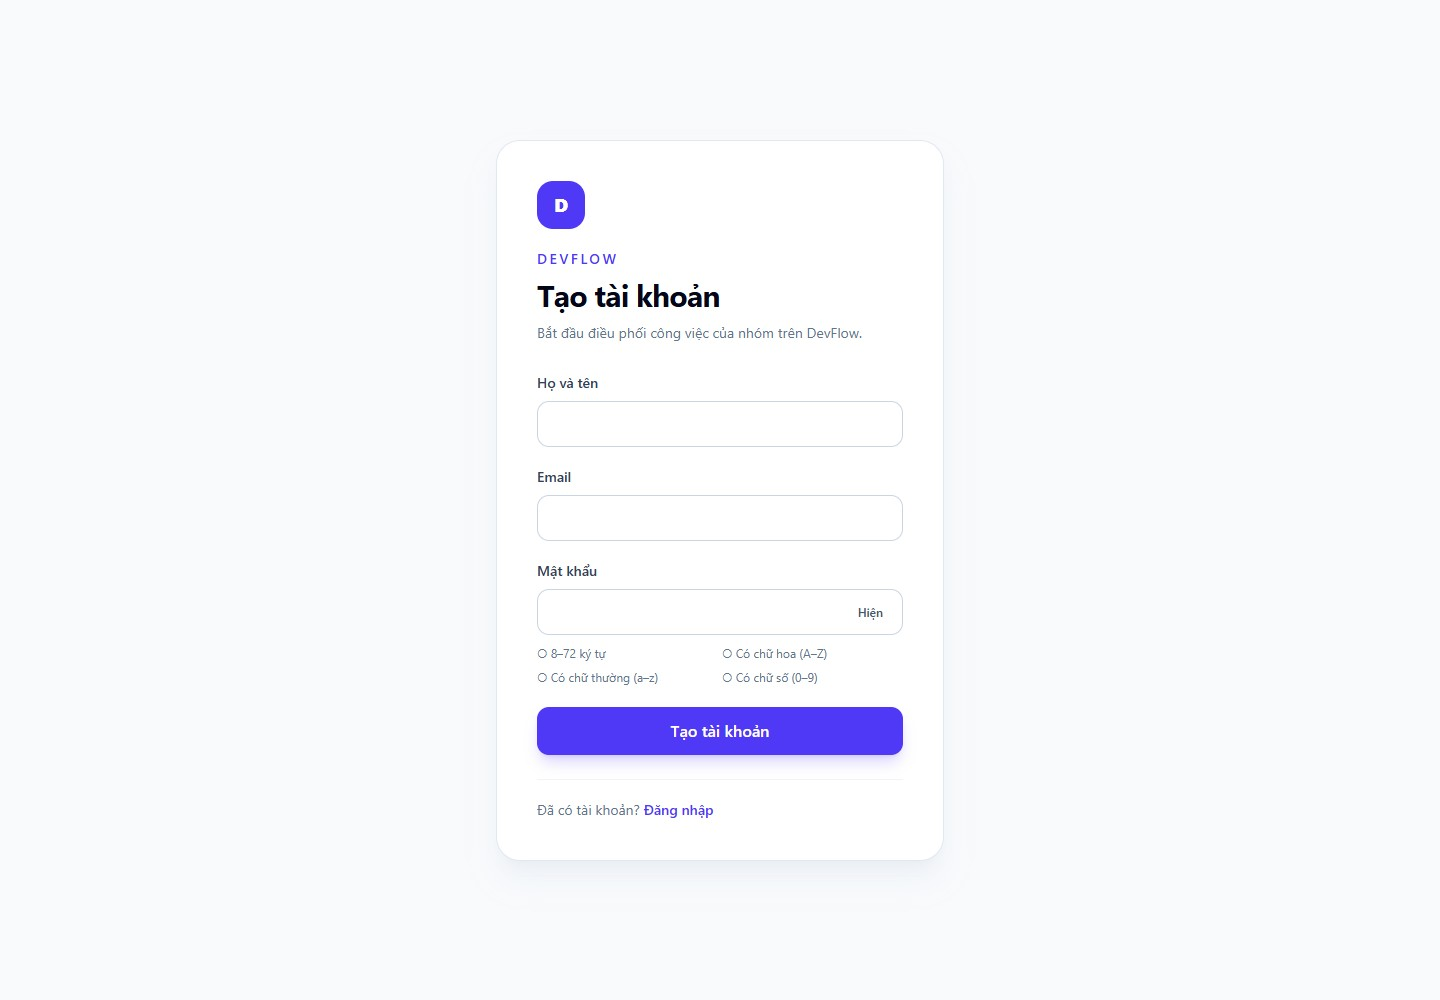
\includegraphics[width=0.78\textwidth]{images/devflow-register.jpg}
    \caption{Biểu mẫu đăng ký tài khoản DevFlow.}
\end{figure}

\begin{figure}[H]
    \centering
    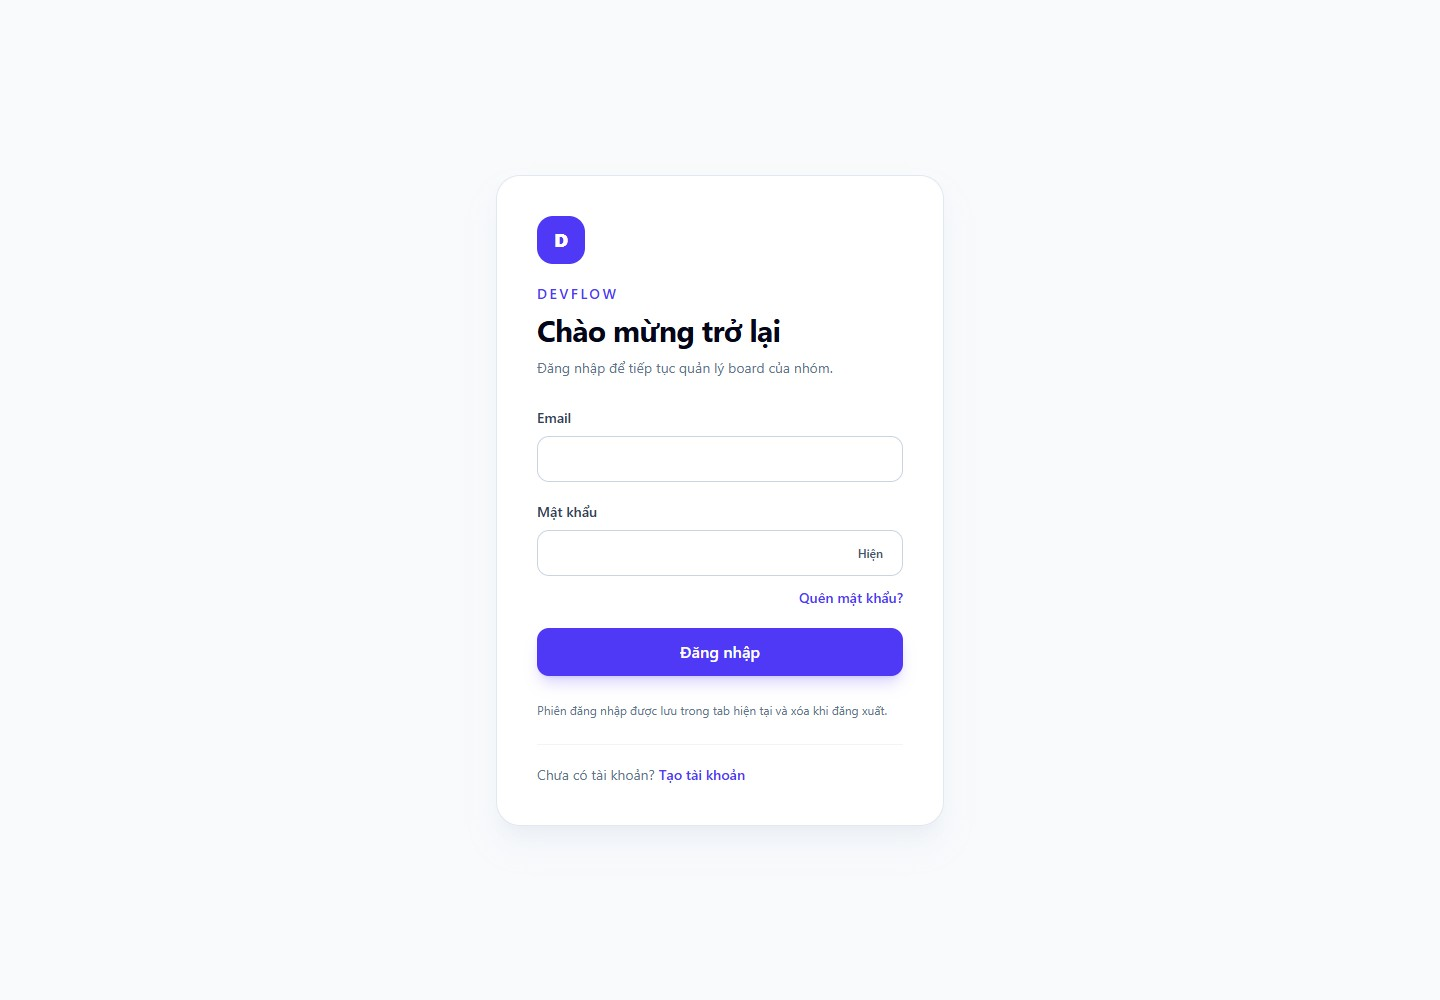
\includegraphics[width=0.78\textwidth]{images/devflow-login.jpg}
    \caption{Màn hình đăng nhập DevFlow.}
\end{figure}

\begin{figure}[H]
    \centering
    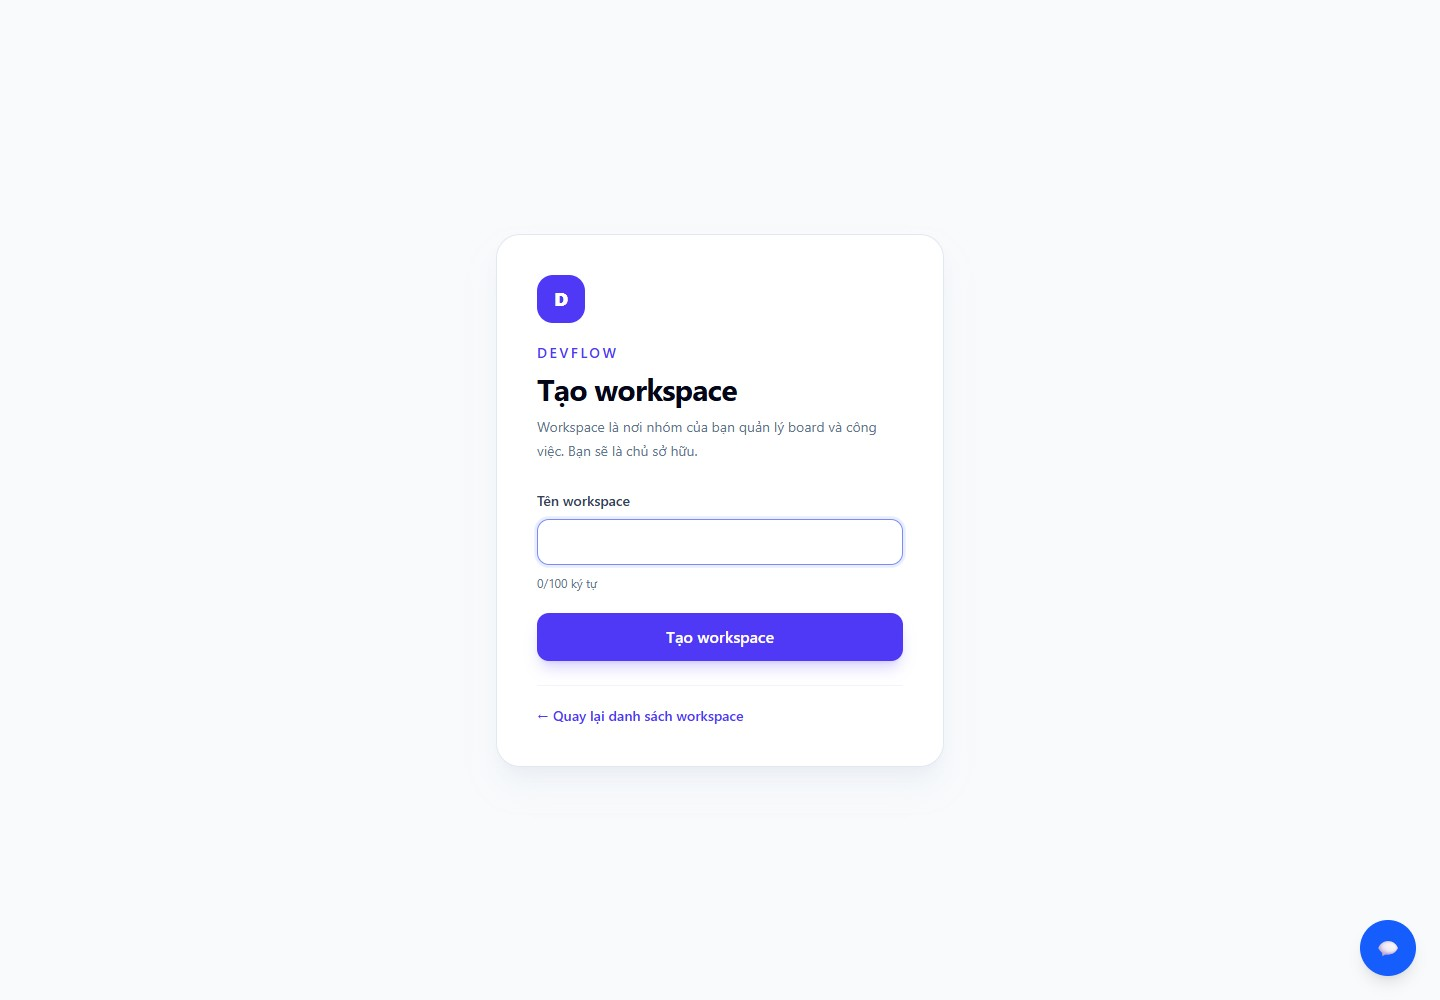
\includegraphics[width=0.78\textwidth]{images/devflow-workspace-create.jpg}
    \caption{Biểu mẫu tạo workspace cho nhóm dự án.}
\end{figure}

\begin{figure}[H]
    \centering
    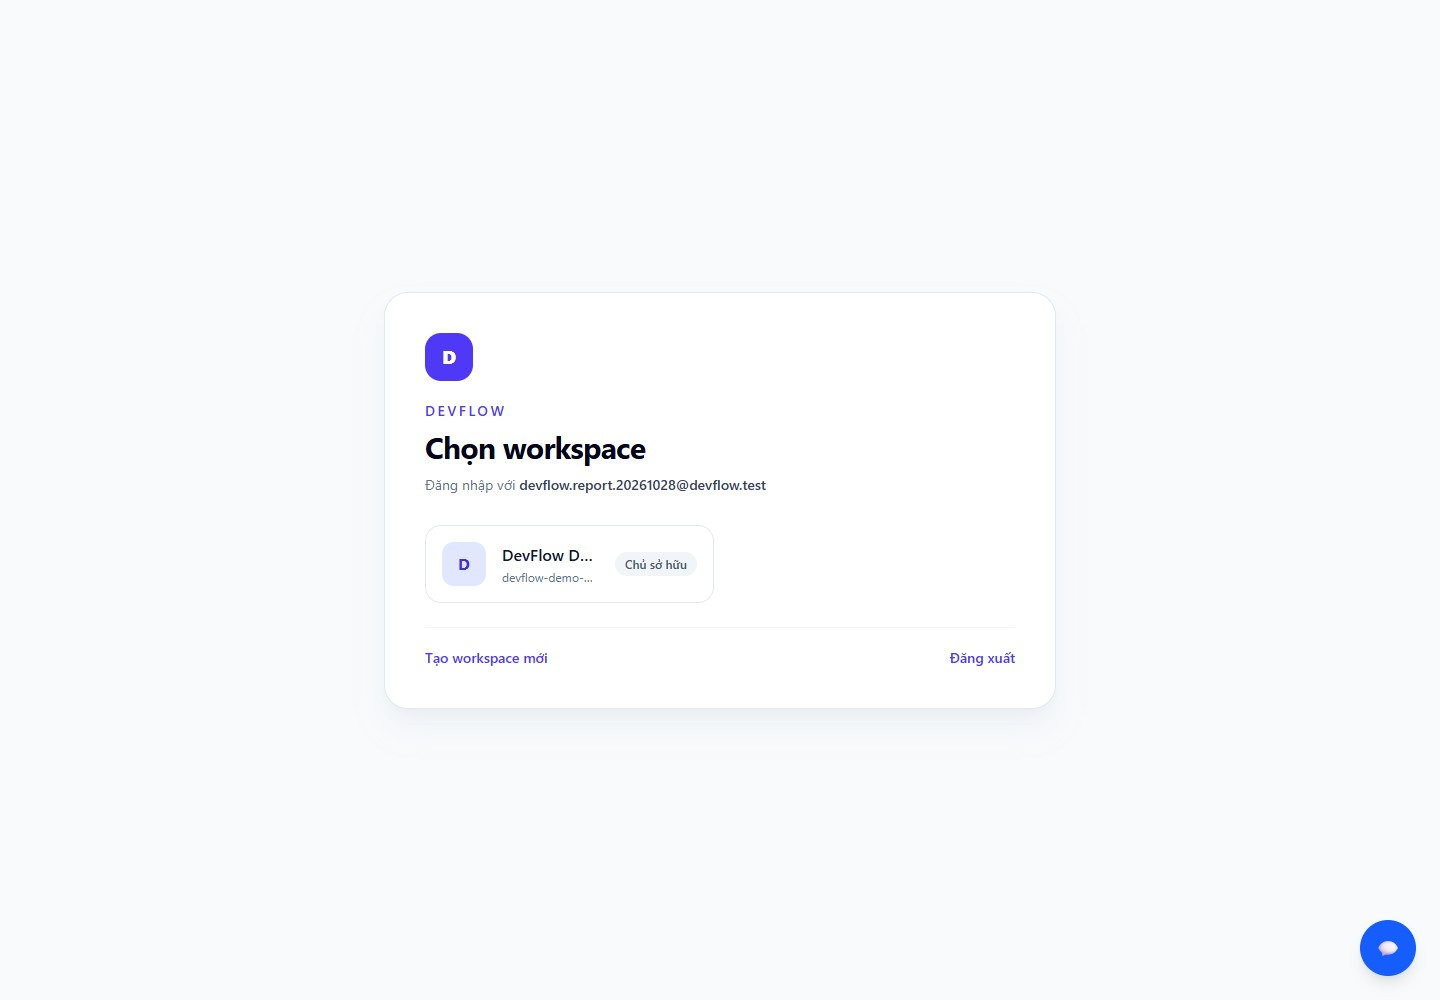
\includegraphics[width=0.78\textwidth]{images/devflow-workspaces.jpg}
    \caption{Danh sách workspace của tài khoản demo.}
\end{figure}

\begin{figure}[H]
    \centering
    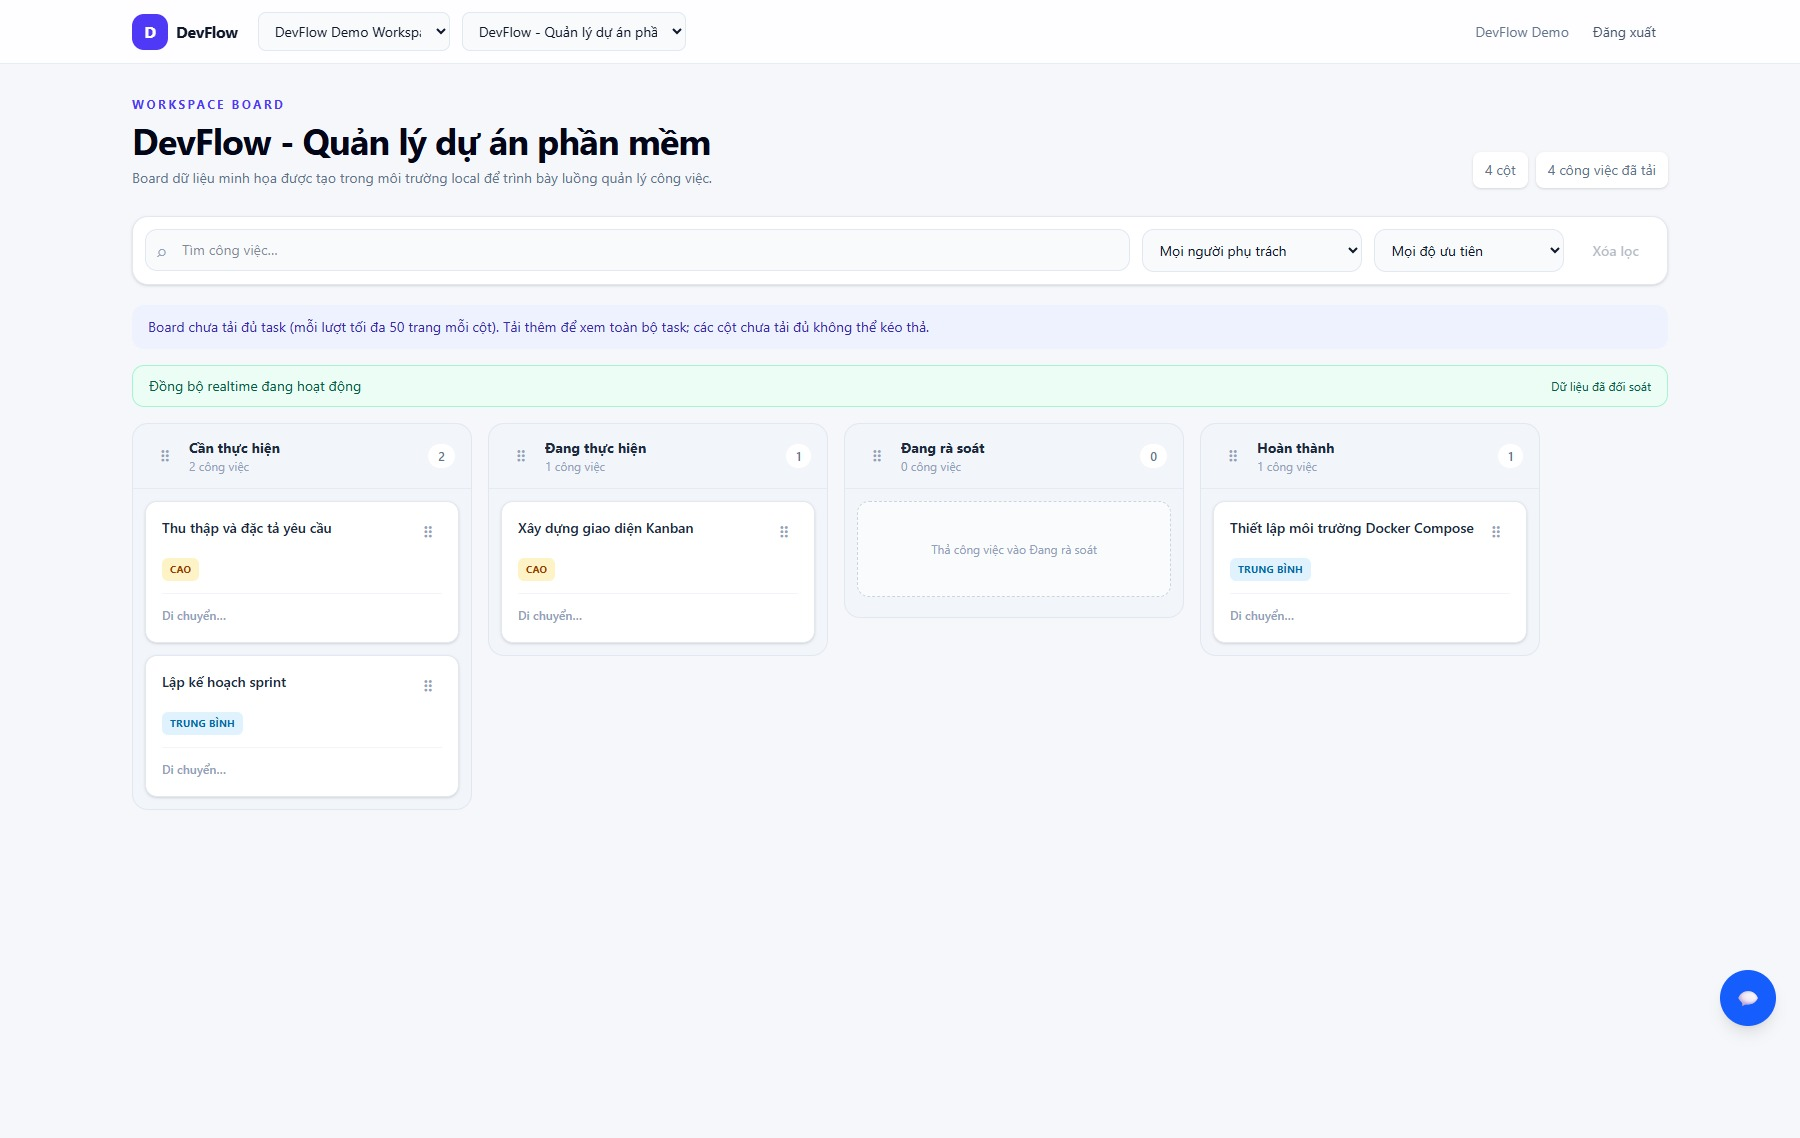
\includegraphics[width=0.96\textwidth]{images/devflow-kanban-board.jpg}
    \caption{Board Kanban với các cột trạng thái và thẻ công việc minh họa.}
\end{figure}

\begin{figure}[H]
    \centering
    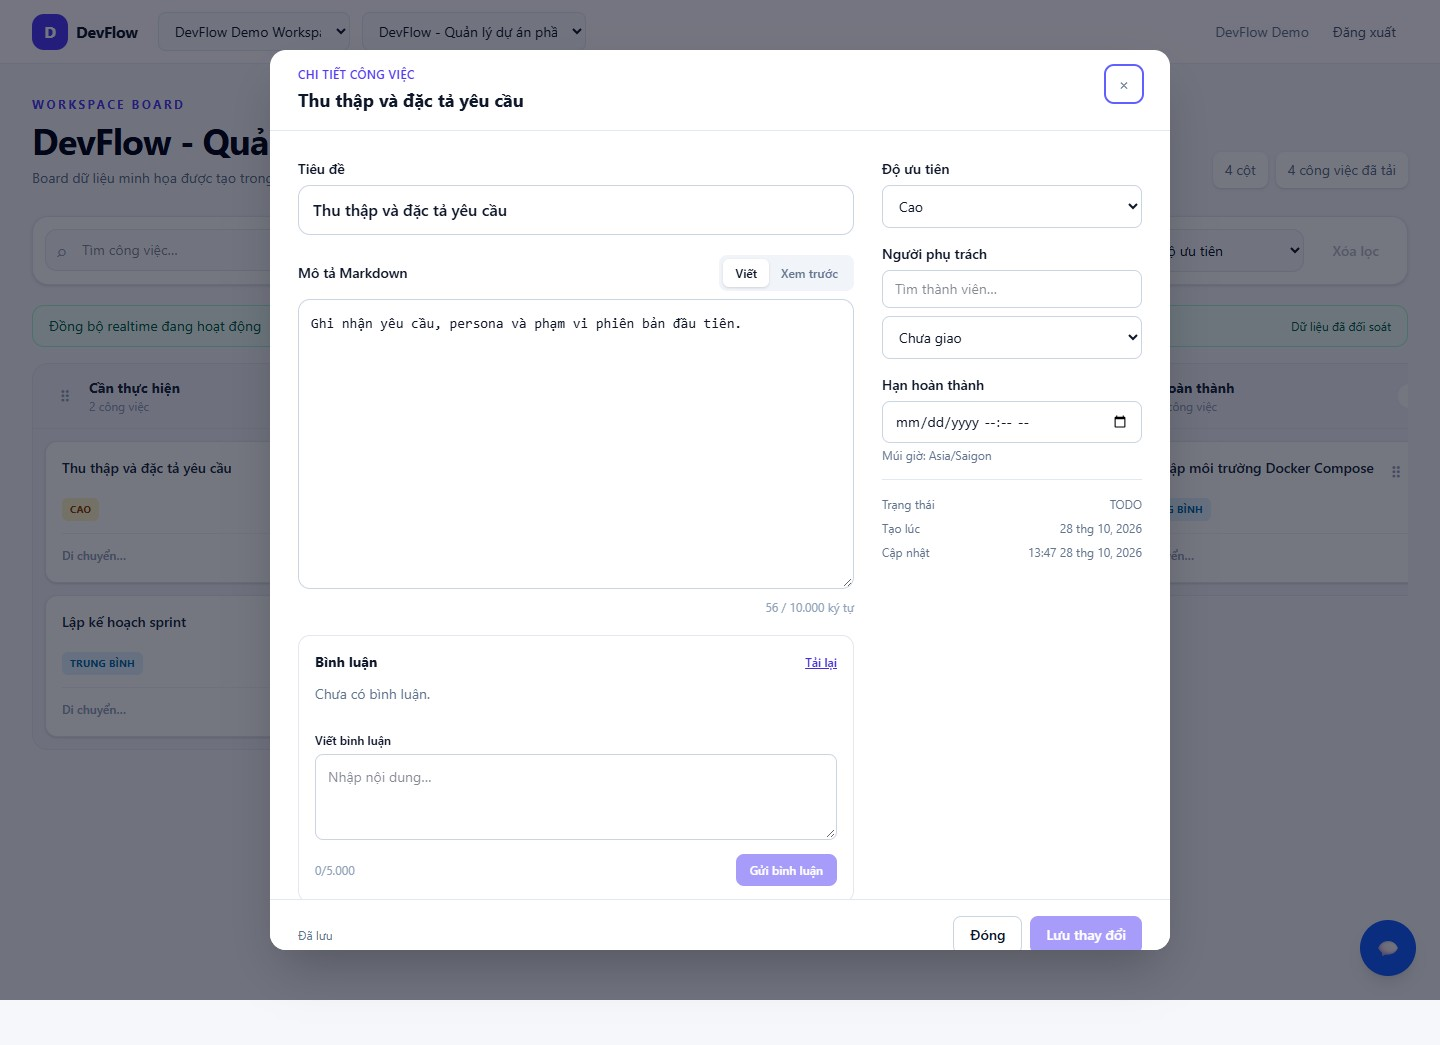
\includegraphics[width=0.96\textwidth]{images/devflow-task-detail.jpg}
    \caption{Cửa sổ chi tiết công việc, mô tả, bình luận và thuộc tính task.}
\end{figure}

\begin{figure}[H]
    \centering
    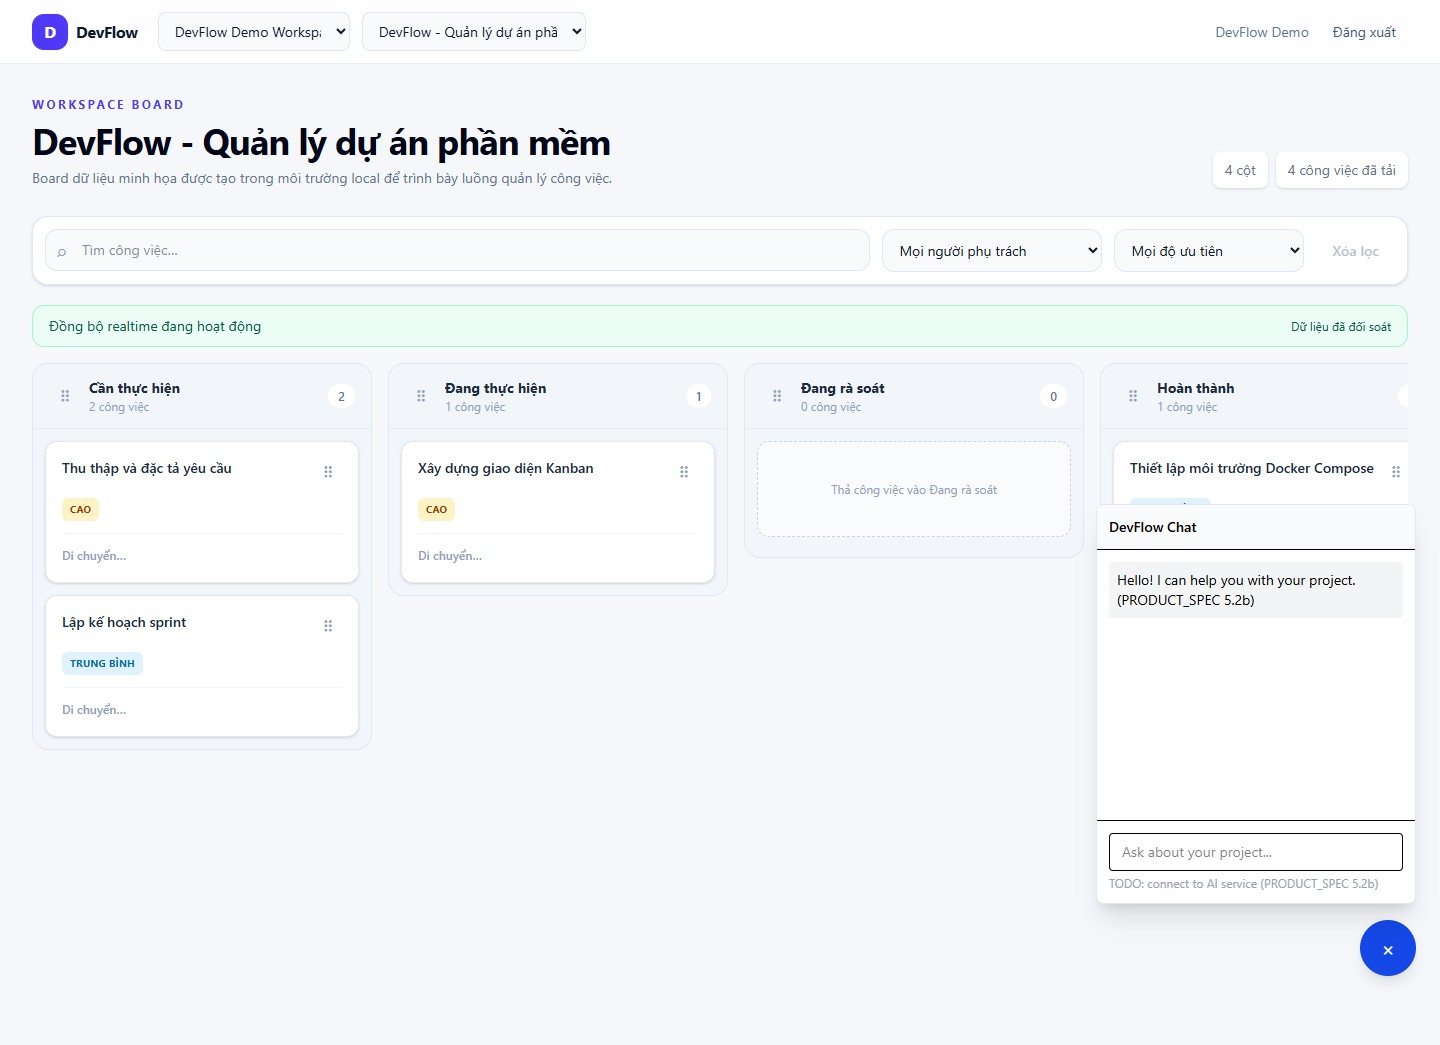
\includegraphics[width=0.78\textwidth]{images/devflow-ai-chat.jpg}
    \caption{Khung DevFlow Chat trên giao diện; kết nối trợ lý AI chưa hoàn thiện.}
\end{figure}

\chapter{TEST CASES VÀ KẾT QUẢ KIỂM THỬ}
\section{Bằng chứng kiểm thử đã lưu}
Hồ sơ tại \texttt{docs/xuan/evidence/T-020/test-summary.json} ghi nhận baseline commit \texttt{4bf5d17}, ngày 15/10/2026. Kết quả gồm 267 backend tests, 0 lỗi/thất bại/bỏ qua; 84 test Git/CI; tác vụ \texttt{check :verifyModuleBoundaries} PASS; frontend \texttt{npm run build} PASS [11]. Đây là kết quả đã lưu cho revision nêu trên, cần chạy lại trên revision bàn giao cuối.

\begin{table}[H]
\centering
\caption{Tóm tắt bằng chứng kiểm thử hiện có}
\begin{tabularx}{\textwidth}{|X|X|X|}
\hline
\textbf{Nhóm kiểm thử} & \textbf{Kết quả được ghi nhận} & \textbf{Giới hạn} \\
\hline
Backend check và module boundary & PASS; 267 test, không có lỗi/thất bại/bỏ qua & Gắn với baseline commit 4bf5d17 \\
Git/CI schema & 84 test; migration, schema, concurrency và query plan & Không đại diện cho toàn bộ luồng Git-to-AI-to-user \\
Frontend build & \texttt{npm run build}: PASS & Hồ sơ không báo cáo E2E production \\
DB query benchmark & P95 34.66 ms với 320 mẫu & DB-only, phụ thuộc host, không phải SLA API \\
AI accuracy / WebSocket latency / production deploy & Chưa có kết quả đo được trong hồ sơ đã rà soát & Cần bổ sung trước nghiệm thu cuối \\
\hline
\end{tabularx}
\end{table}

\section{Các kiểm thử cần bổ sung trước nghiệm thu}
\begin{enumerate}
    \item Chạy backend \texttt{./gradlew check :verifyModuleBoundaries} và frontend \texttt{npm run lint} cùng \texttt{npm run build} trên revision bàn giao.
    \item Thực hiện E2E: đăng nhập, tạo board/task, cập nhật realtime, tiếp nhận webhook, liên kết task, hiển thị CI, yêu cầu AI và kiểm tra phân quyền.
    \item Đo P95 API và WebSocket trên môi trường được mô tả; lưu số mẫu, tải, cấu hình và kết quả.
    \item Đánh giá CI summarizer bằng bộ log có nhãn, tiêu chí chấm và báo cáo độ chính xác; không suy ra từ vài ví dụ demo.
    \item Lưu test reports, link CI và kết quả kiểm tra production vào checklist T-045.
\end{enumerate}

\chapter{HƯỚNG DẪN CÀI ĐẶT VÀ SỬ DỤNG}
\section{Yêu cầu môi trường}
Repo định nghĩa backend Java 17/Spring Boot, frontend Node.js, PostgreSQL 17 và Docker Compose. Cần cài Git và Docker với Docker Compose plugin; các secret AI và CAPTCHA nếu dùng phải được cung cấp qua biến môi trường theo cấu hình dự án, không ghi vào mã nguồn [4], [5].

\section{Khởi chạy local bằng Docker Compose}
Từ thư mục gốc repo, chạy:
\begin{verbatim}
docker compose up -d --build
docker compose ps
\end{verbatim}
Compose khởi chạy PostgreSQL, backend, frontend, Prometheus và Grafana. Các địa chỉ local được cấu hình trong repo gồm:
\begin{itemize}
    \item Frontend: \url{http://localhost:3000}
    \item Backend health: \url{http://localhost:8080/actuator/health}
    \item PostgreSQL: \texttt{localhost:5432}, database \texttt{devflow}
    \item Prometheus: \url{http://localhost:9090}
    \item Grafana: \url{http://localhost:3001}
\end{itemize}
Nếu backend chưa healthy, kiểm tra log bằng \texttt{docker compose logs backend}; kiểm tra database bằng \texttt{docker compose logs db}. Cấu hình local trong compose chỉ phục vụ phát triển, cần thay secret và cấu hình bảo mật riêng trước khi đưa ra Internet.

\section{Tắt môi trường}
Khi kết thúc, chạy:
\begin{verbatim}
docker compose down
\end{verbatim}
Lệnh này dừng các container; dữ liệu PostgreSQL nằm trong named volume để sử dụng lại. Chỉ xóa volume khi thực sự muốn reset dữ liệu môi trường local.

\section{Luồng sử dụng chính}
Đăng ký/đăng nhập, chọn hoặc tạo workspace, mở board, tạo task và cập nhật thông tin; sau đó theo dõi hoạt động Git/CI và các chức năng AI đã được bật trong cấu hình. Tính năng phụ thuộc nhà cung cấp bên ngoài chỉ hoạt động khi credentials tương ứng được cấu hình. Hướng dẫn này mô tả môi trường local; không phải thông tin truy cập production.

\end{document}
